\section{CASE STUDY: OPTIMAL HEATING SYSTEM SCHEDULING}
\label{S:realCaseStudy}

In this section, we show an application of DPC to a real house located in L'Aquila, Italy. Random forest models for DPC built using historical data from this house are described in Section \ref{SS:randomForestsModels}. 
In Section \ref{SS:energyPlusmodel}, we present the thermal energy model of the building in EnergyPlus, built using historical data, construction layout and materials after spending $\sim3$ months of efforts.
In Section \ref{SS:controllersDPCandBangbang}, we set up the DPC optimization problem and describe the bang-bang control strategy.
Finally, in Section \ref{SS:simulationResults}, the performance of the two controllers are compared in terms of energy saving using the EnergyPlus model.
\textcolor[rgb]{0,0,1}{In particular, in Section \ref{SSS:DisturbancePerfect}, we show that DPC allows an energy saving up to $49.2\%$ with respect to the bang-bang controller while guaranteeing thermal comfort for occupants, considering the perfect knowledge of the weather forecast. 
In Section \ref{SSS:DisturbanceUncertain}, we show that DPC is robust with respect to imperfect weather forecast.}
The section organization is graphically shown in Figure \ref{F:overview}.
\begin{figure}[h!]
	\begin{center}
		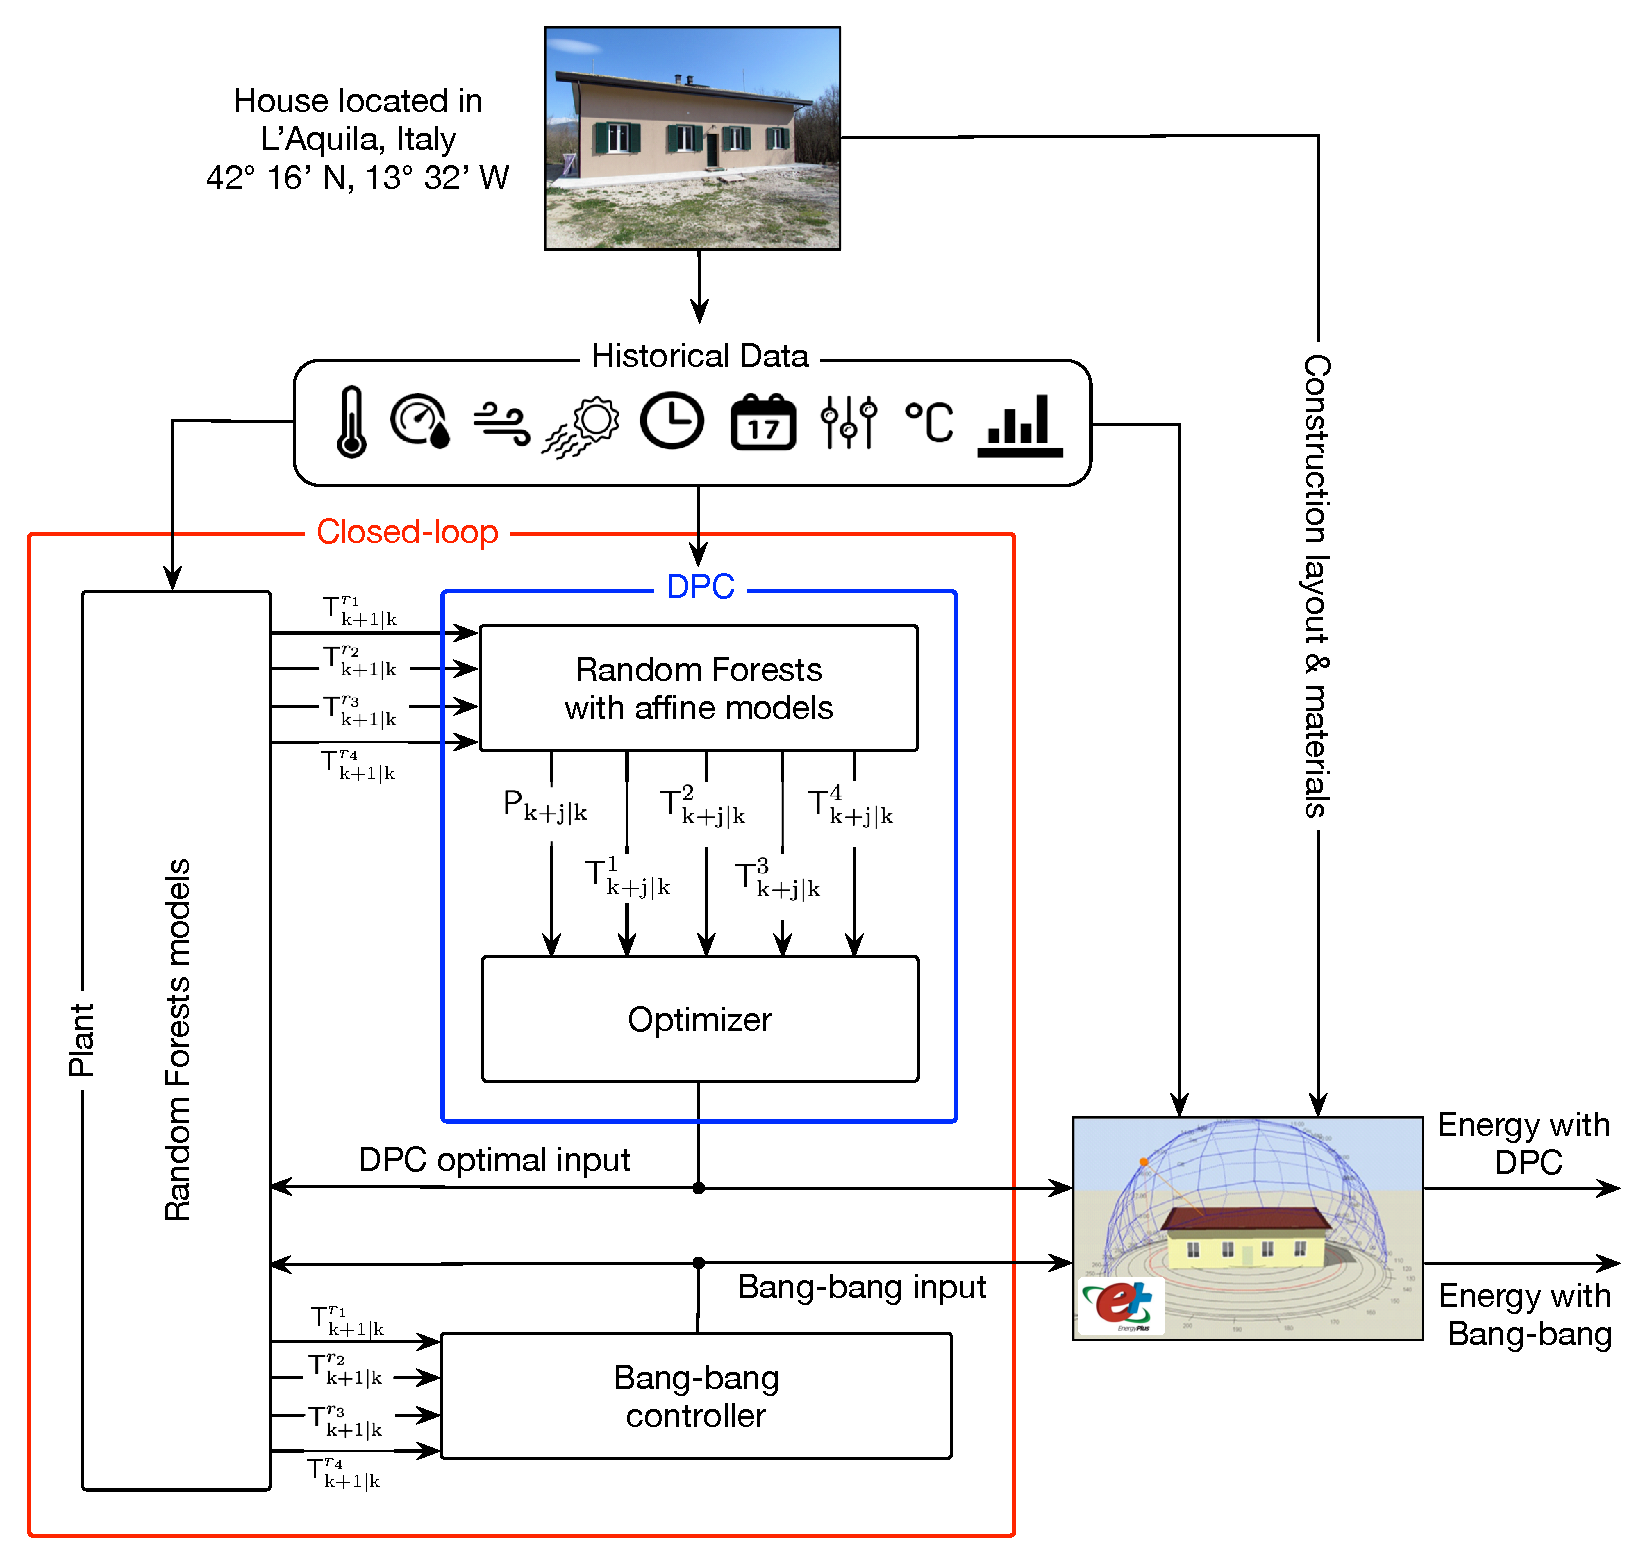
\includegraphics[width=1\linewidth]{figures/overview.eps}
		\caption{Random Forest trained on all features including the control variable are used as the plant in the closed-loop simulations with DPC and bang-bang controller. DPC optimzation uses Random Forests with affine functions as predictive models. Controllers' strategies are evaluated using the EnergyPlus model to compare the actual energy consumption.}
		\captionsetup{justification=centering}
		\label{F:overview}
	\end{center}
\end{figure}

\textcolor[rgb]{0,0,1}{The contribution of this section with respect to Sections \ref{S:casestudy} is threefold:
\begin{enumerate}
	\item we consider experimental data from a lived house, hence subject to real world imperfections, such as random (non predictable) occupancy schedules, open/close windows, random (non predictable) light on/off switch, etc..
	On the other hand, the EnergyPlus model considered in Section \ref{S:casestudy}, although provides an accurate model of a building, is still a simulated model that does not take into account the aforementioned imperfections;
	\item we modify the DPC algorithm to take into account uncertainties on the weather forecast, so making DPC robust with respect to prediction errors;
	\item in Section \ref{S:casestudy}, we want to cut the peak of the power in a specific time range while keeping the temperature as close as possible to a specific setpoint.
	Differently, in this section, we show the adaptability of DPC to different problems, minimizing the energy consumption required to keep room temperatures within a specified range of comfort for an arbitrary amount of time. In this way we show the potential of DPC for energy saving on a long period. 
\end{enumerate}}
\subsection{Description of the house}\label{SS:descriptionHouse}
The chosen case study is a detached off-grid two-story residential house, located in the outskirt of L'Aquila (coordinates $42\degree$ $16'$ latitude and $13\degree$ $32'$ longitude), Italy and is shown in Figure \ref{F:house}. The building, inhabited by the two owners, has a main north-south orientation and it is composed by a heated ground floor and an attic without heating system. Therefore, although the gross area of the house is equal to $209.5\,m^2$, the heated gross area is equal to $112.4\,m^2$.
Thanks to the off-grid characteristic, the technological plants guarantee the complete energy self-sufficiency of the building. The house is equipped with a biomass boiler, a solar thermal plant, a stand-alone photovoltaic system, black water and rainwater reuse systems and a well for water supply, and has complete independence from the utilities.   
The bearing structure of the house is made of reinforced concrete and EPS (expanded polystyrene) insulation, while the building envelope is composed by prefabricated wood-cement blocks, shown in Figure \ref{F:houseSection}, with EPS and graphite insulation, that allow low thermal fluxes. The thermal performance of a wood-cement block, with similar geometry, was investigated in a previous work \cite{Nardi2016}, both with experimental and numerical approach.
The heating system of the building, that supplies the thermal energy required in winter season, is a hydronic system consisting of a vegetable biomass boiler, with a manual ON/OFF, a constant-flow pump station, and tubular steel radiators as shown in Figure \ref{F:housePlantScheme}. The standard biomass boiler has an efficiency of $83.5\%$ with $16.5\ kW$ of thermal power transferred to the water, without gas-flame modulation. The heat transfer fluid distribution is realized through a manifold circuit, that supplies the radiators placed in the various rooms of the house. The energy needs for the domestic hot water (DHW) are covered by the same boiler, coupled with a solar thermal plant. It is worth noting that, in this work, the thermal energy needed for the domestic hot water production is neglected. 
\begin{figure}[t!]
	\begin{center}
		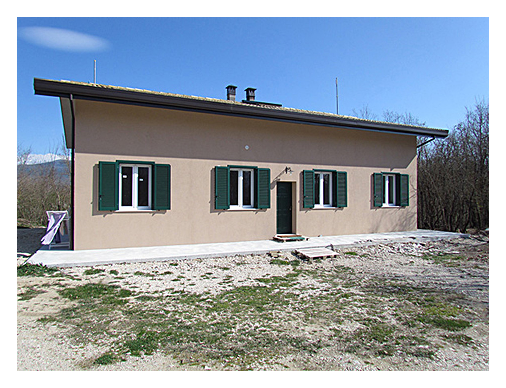
\includegraphics[width=20pc]{figures/Vista_sud.eps}
		\caption{Off-grid residential house.}
		\captionsetup{justification=centering}
		\label{F:house}
	\end{center}
%	\vspace{-0.5cm}
\end{figure}
\begin{figure}[h!]
	\begin{center}
		\subfigure[Walls.]{
			\label{F:houseSection1}
			\centering
			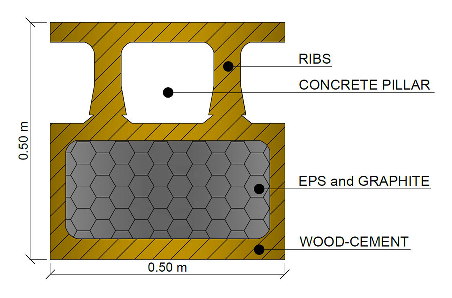
\includegraphics[width=16pc]{figures/blocco_parete_rev01.eps}
		}
		\subfigure[Floor and roof.]{
			\label{F:houseSection2}
			\centering
			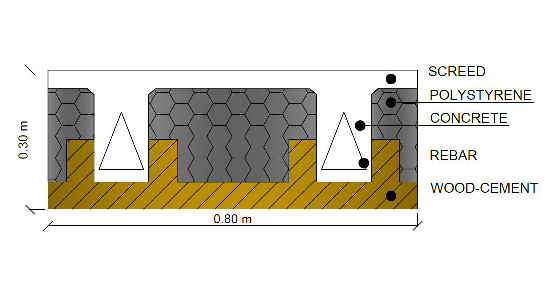
\includegraphics[width=17pc]{figures/blocco_solaio_rev01.eps}
		}
	\end{center}
	\vspace{-0.5cm}
	\caption{Cross-sections of the wood-cement blocks.}
	\captionsetup{justification=centering}
	\label{F:houseSection}
\end{figure}
For a thorough knowledge of the building thermal behavior, an in-situ analysis was carried out. Temperature measuring devices, completely self-produced at the “G. Parolini Lab” of the University of L'Aquila \cite{Pantoli2017}, mainly based on an $ATmega 2560$ microcontroller and $DS18B20$ temperature probes (temperature range from $-55.0\degree C$ to $125.0\degree C$ with an accuracy of $\pm 0.5\degree C$), were employed to acquire the ambient temperatures of $4$ differently oriented rooms of the house as shown in Figure \ref{F:houseFloors} (displayed with red dots $A1$, $A2$, $A3$ and $A4$). The probes positions were chosen to optimize the data acquisition and to minimize the discomfort of the occupants in the house. Furthermore, as can be seen in Figures \ref{F:housePlantScheme} and \ref{F:houseFloors}, a commercial heat meter (temperature range from $10.0\degree C$ to $90.0\degree C$ with an accuracy of $\pm 0.05\degree C$, displayed with orange dot $G1$) was installed downstream of the biomass boiler to measure the produced thermal energy. The turbine flowmeter was installed on the return pipe, while the two thermocouples were placed inside the delivery and return pipes, respectively. All the measuring devices have been set with a data acquisition rate equal to $10$ minutes, from March $11^{th}$ $2016$ to May $15^{th}$ $2016$.

The collected data are used in the following to create both an EnergyPlus and a random forest model for the energy consumption assessment of the house. These models will be used for performance comparison of DPC with respect to a classical bang-bang controller. In particular DPC will be set up to provide an optimal ON/OFF scheduling policy for the heating system in order to save energy while guaranteeing thermal comfort for the occupants. To this aim, we also create random forest models for power consumption and room temperatures to be used in the closed-loop simulations. 

\begin{figure}[t!]
	\begin{center}
		\includegraphics[width=27pc]{figures/Schema_di_impianto.eps}
		\caption{Technological plant scheme of the use case.}
		\captionsetup{justification=centering}
		\label{F:housePlantScheme}
	\end{center}
\end{figure}
\begin{figure}[t!]
	\begin{center}
		\subfigure[Ground floor.]{
			\label{F:houseGroundFloor}
			\centering
			\includegraphics[width=26pc]{figures/Arch_PT_e_sonde.eps}
		}
		\subfigure[Attic.]{
			\label{F:houseAttic}
			\centering
			\hspace{-1.6cm}
			\includegraphics[width=22.8pc]{figures/Arch_P1.eps}
		}
	\end{center}
	\caption{Layout of the house and probes placement. Legend: red circle for ambient temperature; orange circle for heat meter.}
	\captionsetup{justification=centering}
	\label{F:houseFloors}
\end{figure}
\subsection{EnergyPlus model}\label{SS:energyPlusmodel}
In this section we create an EnergyPlus model of the thermal energy consumption of the house that will be used in Section \ref{SS:simulationResults} to compare the quality of the DPC with respect to a classical bang-bang controller.

To assess energy performance of the use case heating system, the EnergyPlus \cite{energyPlus} together with DesignBuilder modeling environment \cite{designBuilder} has been employed. The model has been created based  on L'Aquila weather data, shown in Figure \ref{F:houseExternalWeather}, provided by the CETEMPS – Centre of Excellence \cite{CETEMPS}. According to the K\"{o}ppen-Geiger climate classification, Italy is classified in Csa, Cfa and Csb climate zones, with a warm temperate climate \cite{Peel2007}.

Because of the complex morphology of the blocks shown in Figure \ref{F:houseSection}, some simplified assumptions were made, in order to create the EnergyPlus virtual model. Considering the thermal properties of the wood-cement blocks that compose the walls shown in Figure \ref{F:houseSection1}, the thermal effects of the ribs were neglected. For the block employed for floor and roof shown in Figure \ref{F:houseSection2}, a less complex equivalent block, with only three layers, was evaluated in order to consider only one equivalent thermal transmittance value. The properties of the blocks used for the simulation model are listed in Table \ref{T:houseProperties}.    

Therefore, the dynamic simulation model of the use case, shown in Figure \ref{F:houseVirtualModel}, has been created by analyzing the fundamental characteristics of the building (orientation, geometry, structural members, heating system components, air changes with natural ventilation, activity, internal gains, air leakages) and the weather file specifically created for L'Aquila. The comprehensive method was chosen for modeling the heating system, once checked all the characteristics of the components.
\begin{figure}[t!]
	\begin{center}
		\hspace{-0.7cm}
		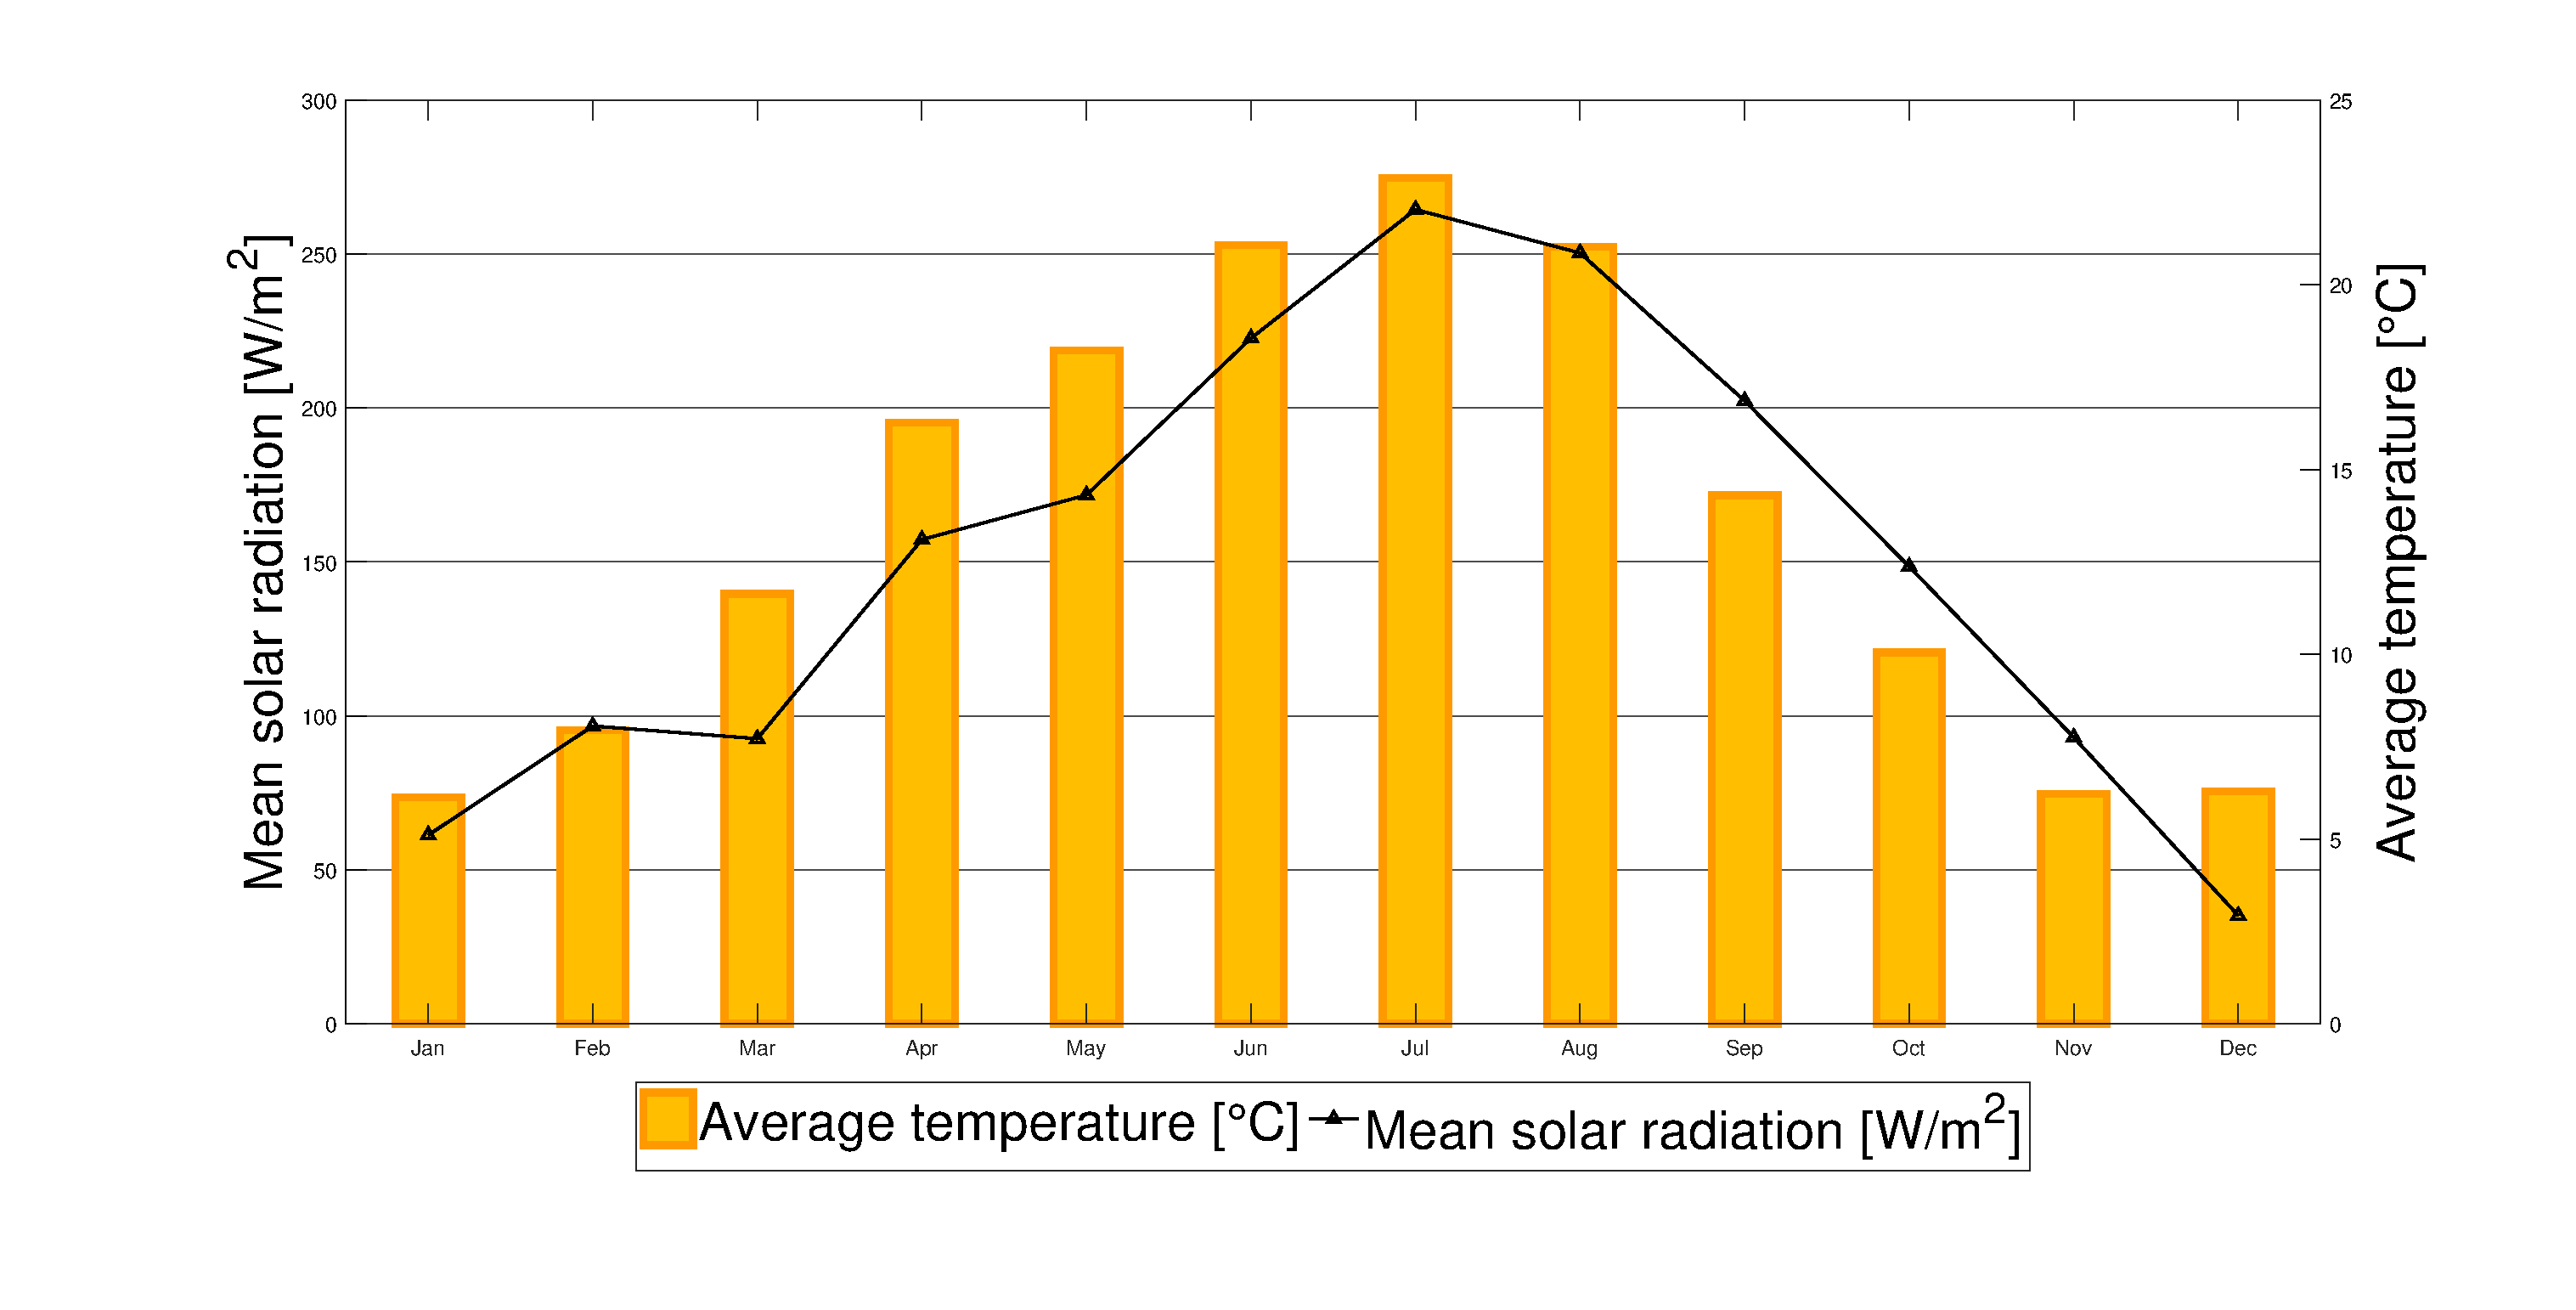
\includegraphics[width=28pc]{figures/dati_climatici_rev01.eps}
		\vspace{-0.5cm}
		\caption{Weather data of L'Aquila, Italy.}
		\captionsetup{justification=centering}
		\label{F:houseExternalWeather}
	\end{center}
\end{figure}
\begin{table}[t!]
	\centering
	\begin{tabular}{ccccc}
		\toprule
		\multirow{3}{1.4cm}{\centering Structural member} & \multirow{3}{3.7cm}{\centering Layer 
			description (from inside to outside)}       & Thermal     		     & Total     & Total        \\
		&                                             & resistance   		     & thickness & U-value      \\
		&                                             & $[(m^2K)/W]$		     & $[m]$     & $[W/(m^2K)]$ \\
		
		
		\midrule
		\multirow{3}*{Wall}                               & Wood-cement                                 & $0.308$     		     &           &              \\ 
		& Concrete                                    & $0.096$    		     & $0.50 $   & $0.12 $      \\ 
		& EPS and graphite                            & $6.774$    		     &           &              \\
		&							                    &						 &		     &			    \\
		
		
		\multirow{3}*{Floor}        					  & Wood-cement                                 & $0.308$     		     &           &              \\ 
		& Polystyrene                                 & $6.000$     		     & $0.23 $   & $0.28 $      \\ 
		& Screed                                      & $0.027$     		     &           &              \\
		&									    	    &					 	 &		     &			    \\
		
		
		\multirow{5}{1.4cm}{\centering Pitched roof} 	  & Wood-cement                                 & $0.308$                &           &              \\ 
		& Polystyrene                                 & $6.000$                &           &              \\
		& Screed                                      & $0.027$                & $0.31 $   & $0.13 $      \\ 
		& \multirow{2}{3.7cm}{\centering Polyurethane 
			resins and polyisocianurate foams}          & \multirow{2}*{$4.000$} &           &              \\
		&                                             &                        &           &              \\
		\bottomrule
	\end{tabular}
	\caption{Wood-cement blocks properties.}
	\captionsetup{justification=centering}
	\label{T:houseProperties}
\end{table}
In order to calibrate the EnergyPlus model, a comparison between simulated and measured thermal energy consumption was performed. Considering the off-grid characteristic of the house, the installation of a heat meter was necessary for acquiring the actual energy consumption. Moreover, the heat meter installation has allowed a detailed knowledge of the actual heating system scheduling, shown in Figure \ref{F:houseActualScheduling}, faithfully reproduced in the simulated model. The heat meter, that consists of two thermocouples for flow and return thermal fluid temperatures, a turbine flowmeter and a controller, employed Equation \eqref{Eq:energyConsumption} to calculate the real thermal energy consumption $\dot Q$ of the house.
\begin{equation}\label{Eq:energyConsumption}
\dot Q = 0.2777698\times10^{-3}\times\rho\times\Delta V\times c_p\times\Delta T
\end{equation}
In \eqref{Eq:energyConsumption} $\dot Q$ is the thermal energy consumption $[Wh]$, $\rho$ is the water density $[kg/m^3]$, $\Delta V$ is the water volume variation $[m^3]$ detected by the turbine flowmeter, $c_p = 4.186\, [kJ/(kgK)]$ is the water specific heat at constant pressure, $\Delta T$ is the difference between flow and return temperatures of the water $[K]$, $0.2777698∙10−3$ is a dimensionless conversion factor. The considered period goes from March $15$, $2016$ to April $15$, $2016$.
\begin{figure}[t!]
	\begin{center}
		\includegraphics[width=20pc]{figures/Render_rev01.eps}
		\caption{Virtual model of the use case.}
		\captionsetup{justification=centering}
		\label{F:houseVirtualModel}
	\end{center}
\end{figure}
\begin{figure}[t!]
	\begin{center}
		\includegraphics[width=28pc]{figures/Scheduling_rev02.eps}
		\caption{Actual scheduling of the heating system, where white color means switched OFF and green color switched ON, and ($T_{ext,ave}$) is the external average temperature. From midnight to $8am$ the heating system is always switched off.}
		\captionsetup{justification=centering}
		\label{F:houseActualScheduling}
	\end{center}
\end{figure}
Following the hourly calibration proposed by the M\&V guidelines of ASHRAE \cite{USDOE}, also applied in \cite{Mustafarai2014,Raftery2011}, a simulated model is calibrated when the mean bias error (MBE) and the coefficient of variation of the root mean square error [CV(RMSE)] are less than acceptable tolerances, respectively equal to $\pm 10.0\%$ and $30.0\%$. MBE and CV(RMSE) have been calculated by using Equations \eqref{Eq:mbe} and \eqref{Eq:cvrmse}.

\begin{equation}\label{Eq:mbe}
MBE(\%) = \frac{\sum_{Period}{(S-M)_{Interval}}}{\sum_{Period}{M_{Interval}}} \times 100
\end{equation}

where $M$ is the measured $kWh$ and $S$ is the simulated $kWh$.

\begin{align}\label{Eq:cvrmse}
\nonumber CV(RMSE_{Period}) &= \frac{RMSE_{Period}}{A_{Period}} \times 100 \\
				            &= \sqrt{\frac{\sum{(S-M)^2_{Interval}}}{N_{Interval}}} \times \frac 1{A_{Period}} \times 100
\end{align}

where $A_{Period}$ is the mean of the measured data for the period, Equation \eqref{Eq:aperiod}, and $N_{Interval} = 4563$ is the number of time intervals in the monitoring period.

\begin{equation}\label{Eq:aperiod}
A_{Period} = \frac{\sum_{Period}{M_{Interval}}}{N_{Interval}}
\end{equation}

The comparison between numerical and experimental data is shown in Figure \ref{F:houseComparisonExperimental} and shows a quite good agreement. Therefore, with a MBE equal to $7.38\%$ and a CV(RMSE) equal to $8.37\%$, the EnergyPlus model of the use case can be considered well calibrated.  
\begin{figure}[t!]
	\begin{center}
		\subfigure[Thermal energy comparison. The accuracy error is $7.38\%$ with MBE definition and $8.37\%$ with CV(RMSE) definition]{
			\label{F:houseComparisonExperimentalEnergy}
			\centering
			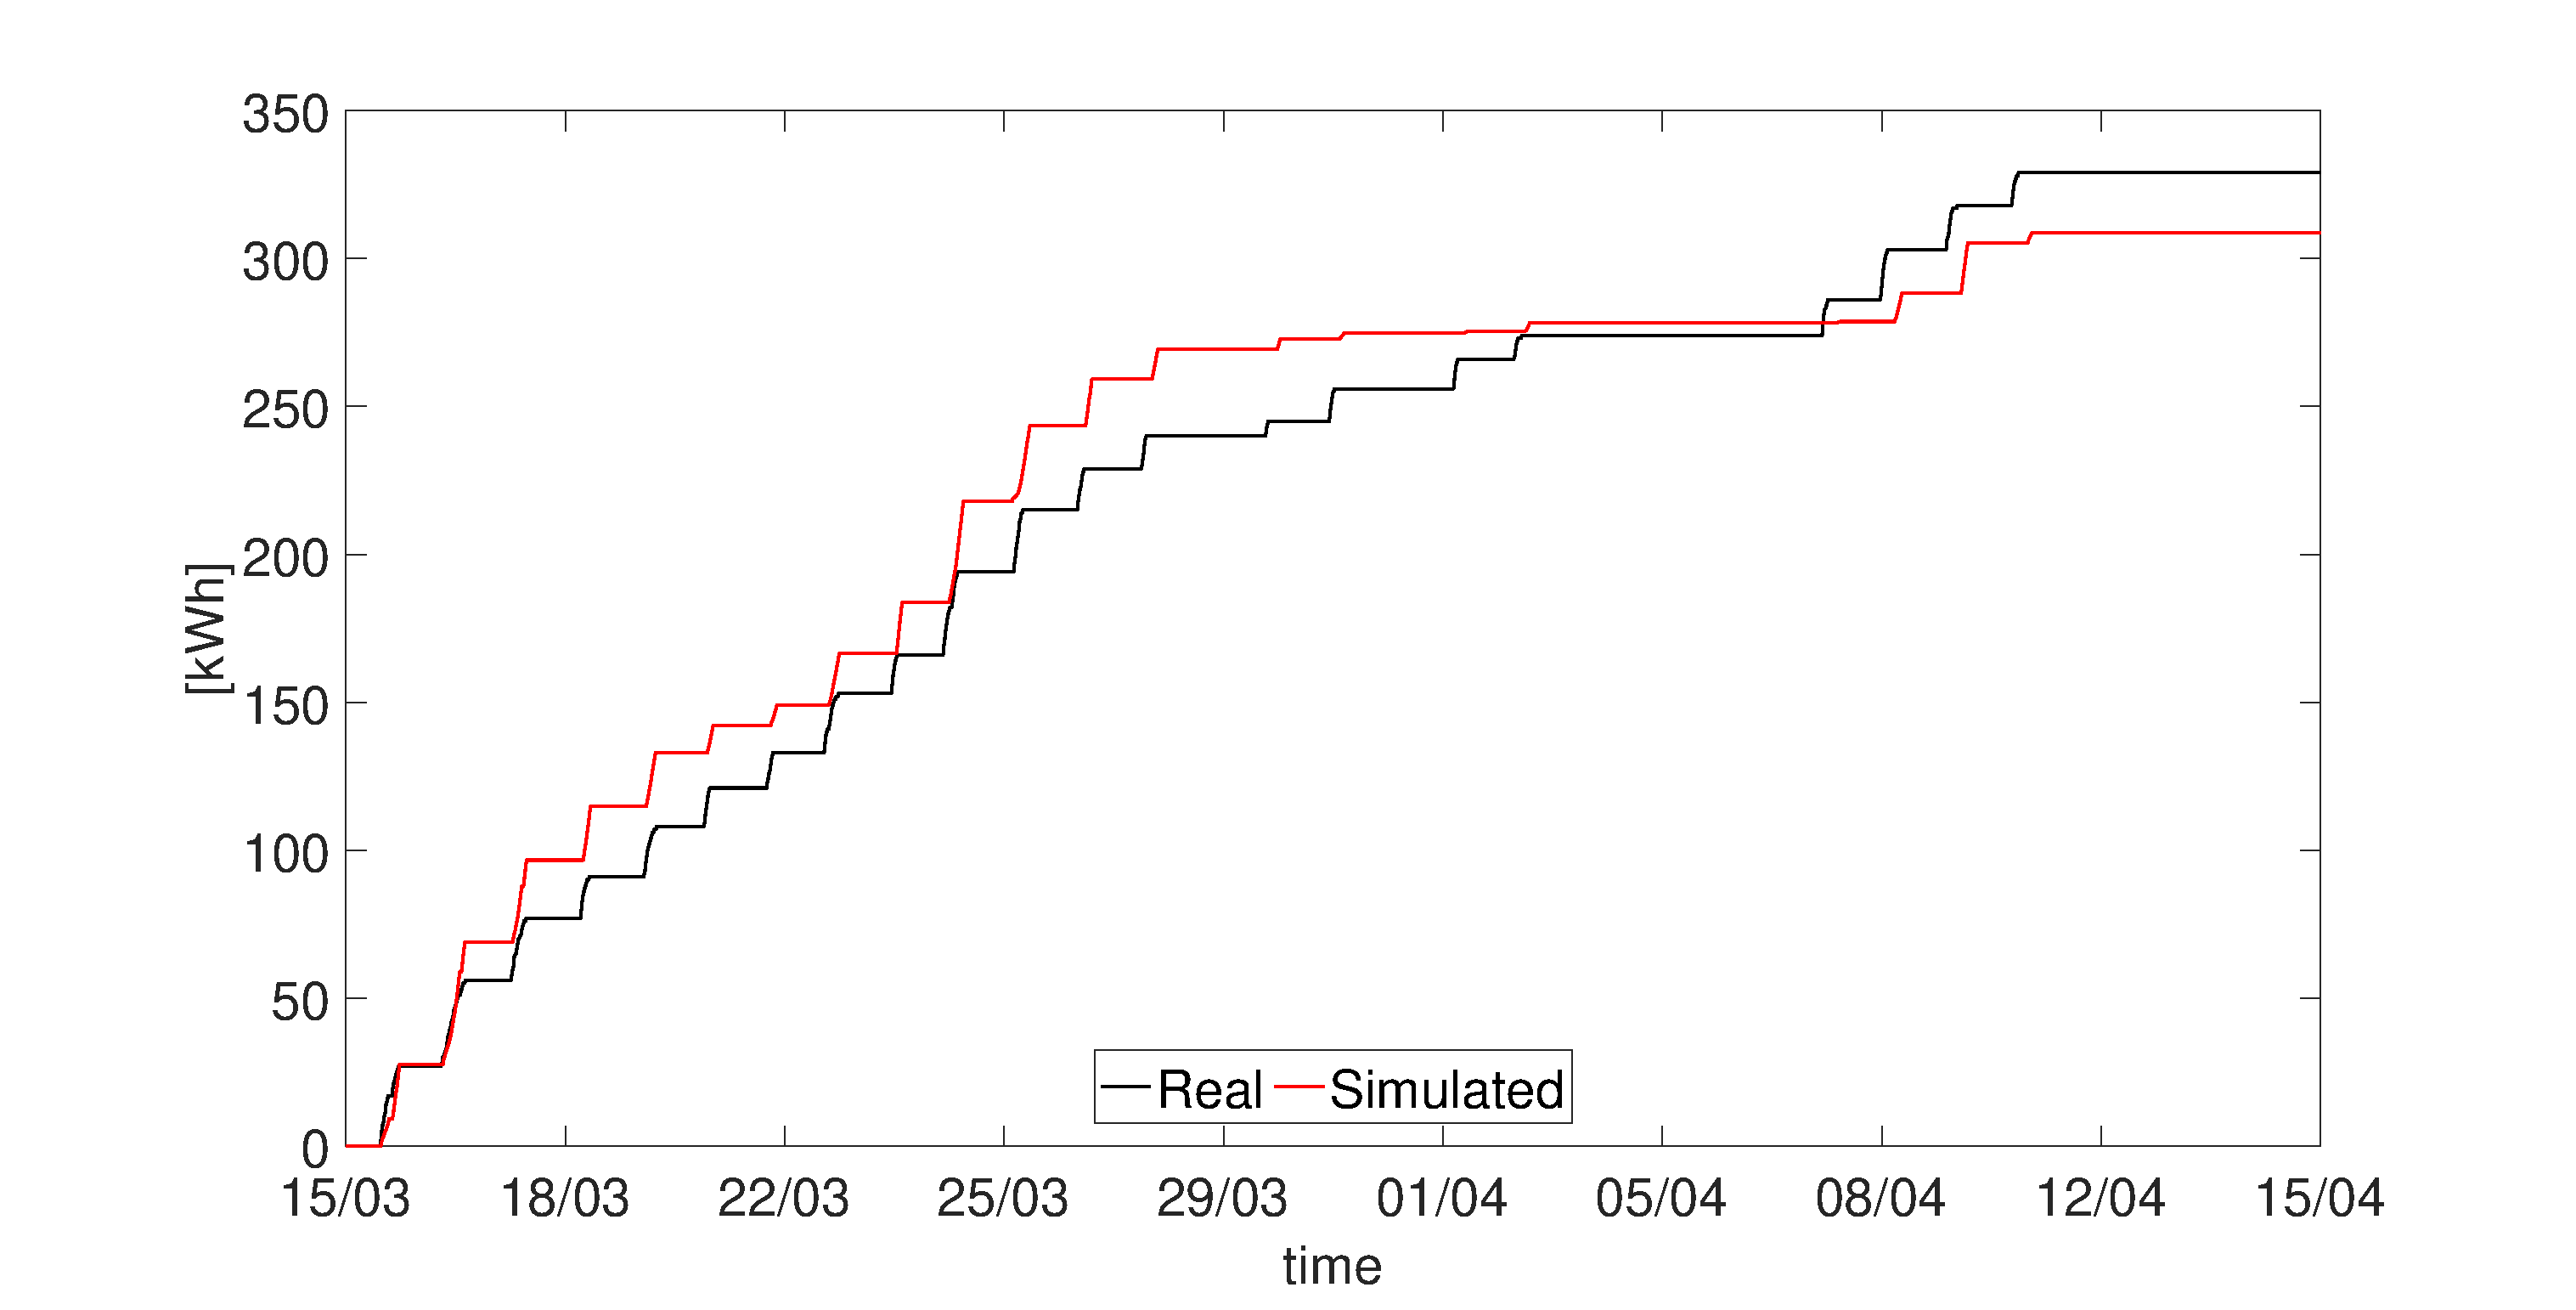
\includegraphics[width=28pc]{figures/Thermal_energy_rev01.eps}
		}
		\subfigure[Thermal power comparison.]{
			\label{F:houseComparisonExperimentalPower}
			\centering
			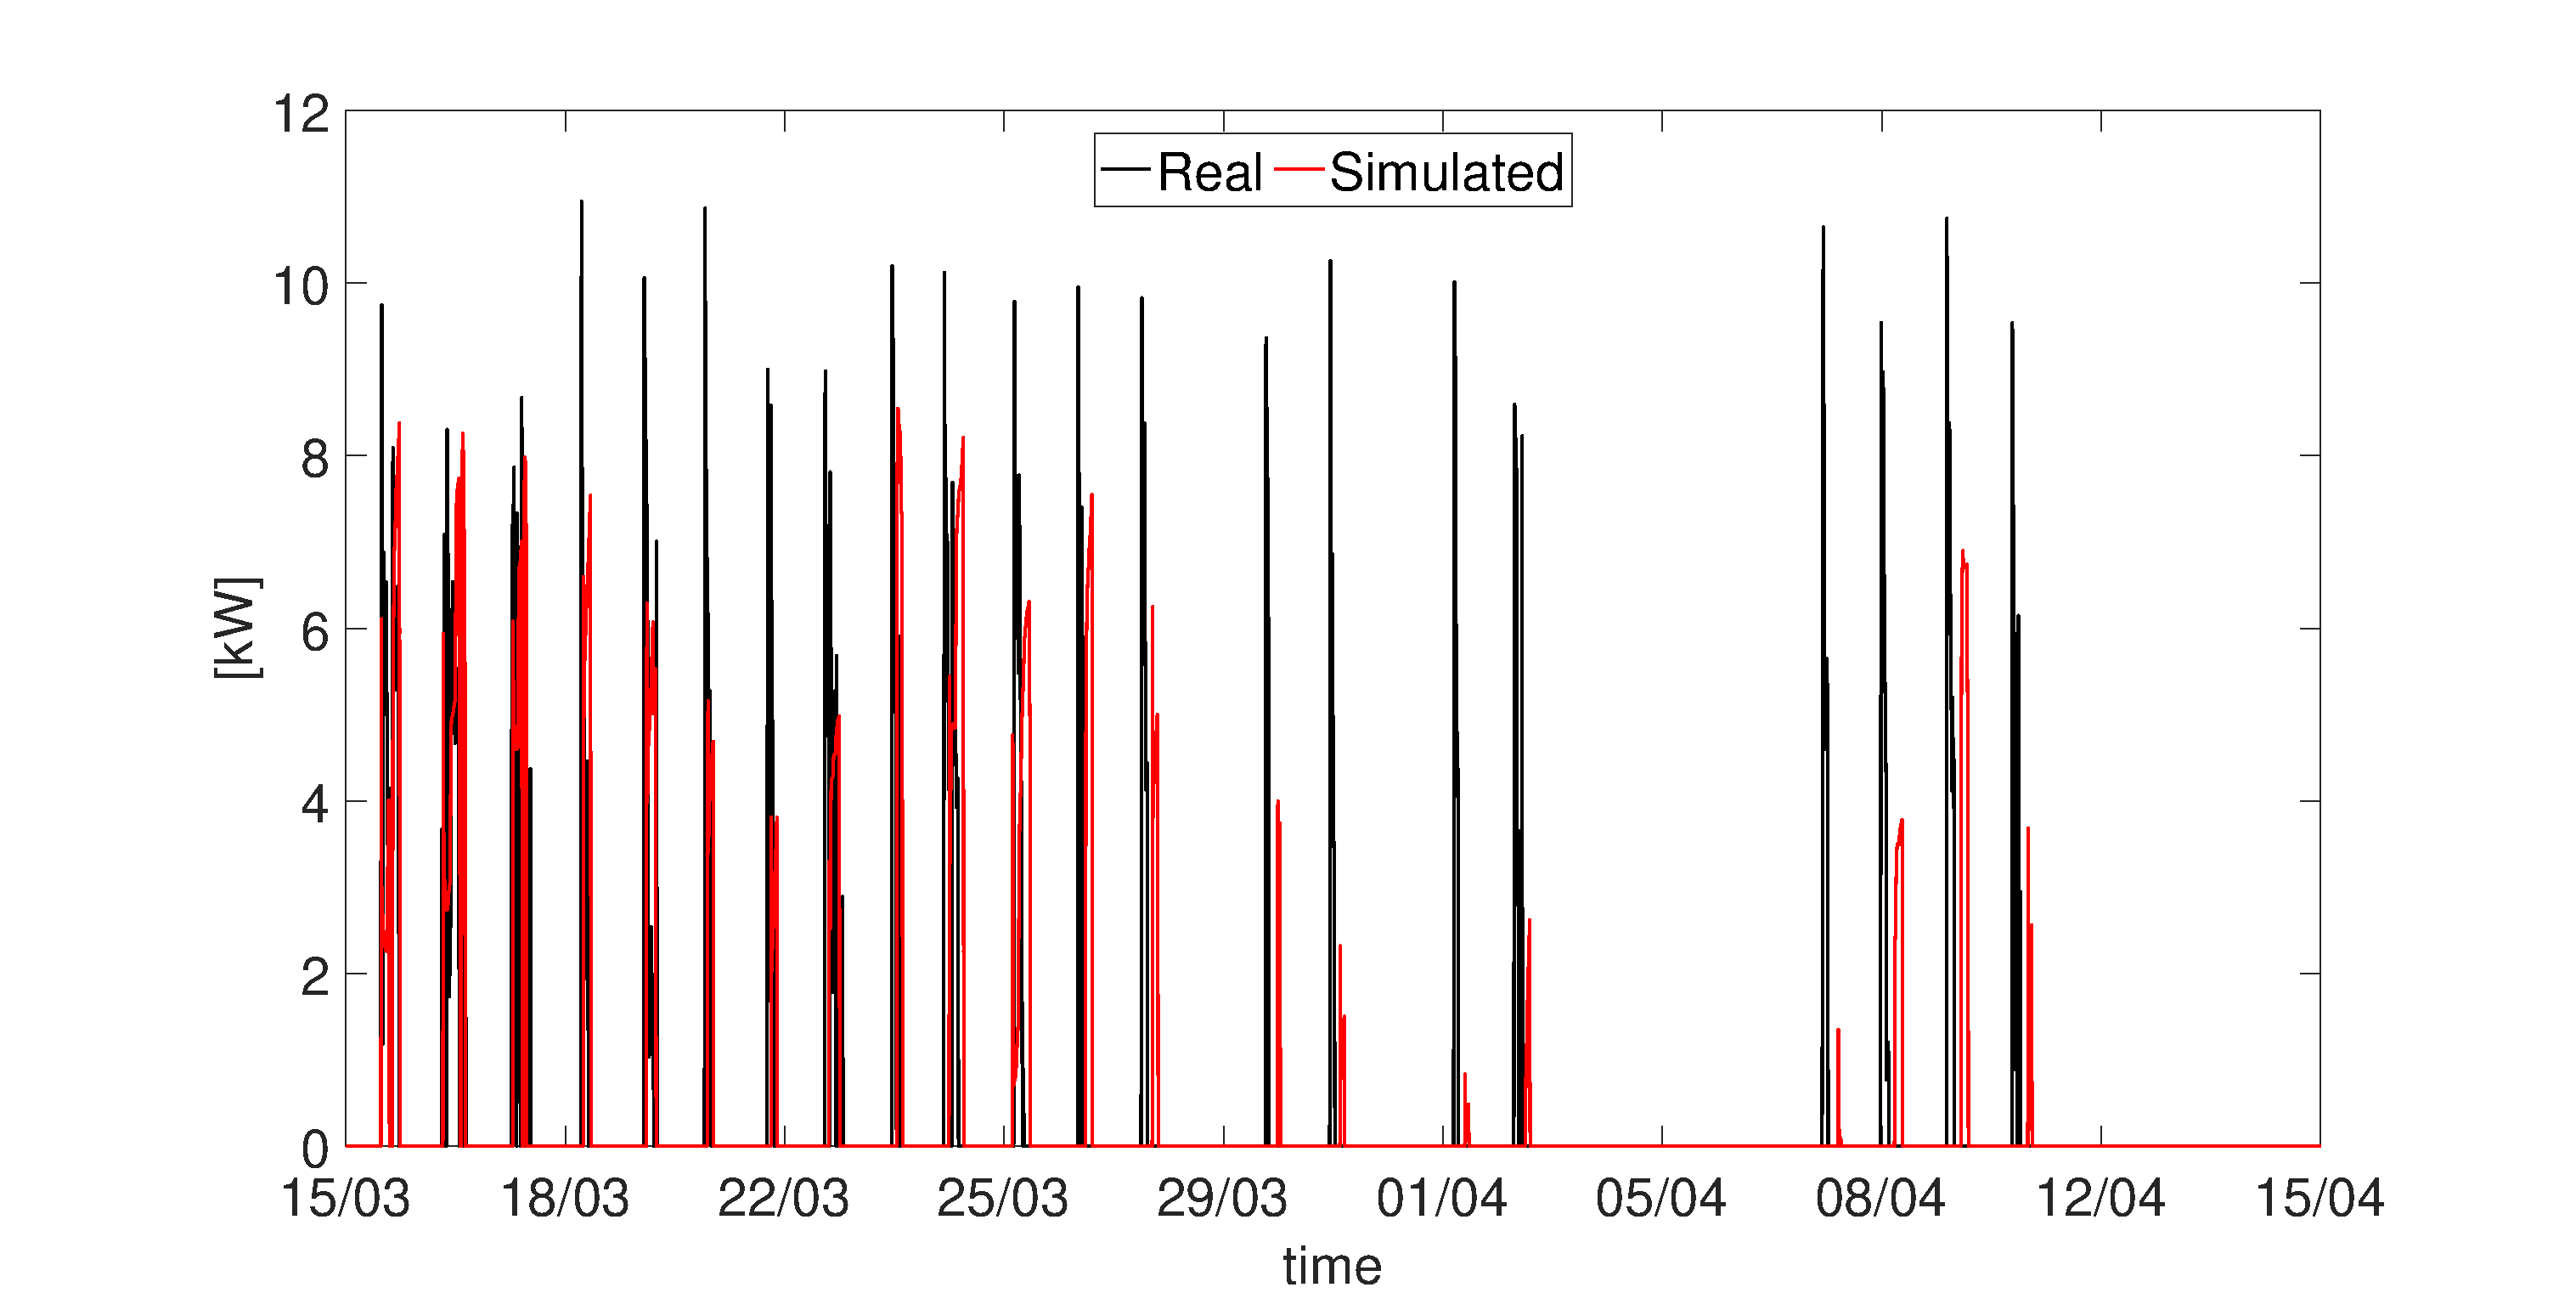
\includegraphics[width=28pc]{figures/Thermal_power.eps}
		}
	\end{center}
	\caption{Comparison between numerical and experimental data.}
	\captionsetup{justification=centering}
	\label{F:houseComparisonExperimental}
\end{figure}
\subsection{Random forest models}
\label{SS:randomForestsModels}
For the closed-loop simulations with DPC we create $2$ different sets of models, $S_1 = \{\tT^{r_1}_{k+j},\tT^{r_2}_{k+j},\tT^{r_3}_{k+j},\tT^{r_4}_{k+j}\}$ and $S_2 = \{\tP_{k+j},\tT^{1}_{k+j},\tT^{2}_{k+j},\tT^{3}_{k+j},\tT^{4}_{k+j},\ j = 1,\ldots,N\}$, using random forests. In each set we have  $4$ models that describe the room temperature evolution ($\tT^{r_i}$ and $\tT^i$, $i=1,2,3,4$) in each of the $4$ rooms equipped with temperature sensors. In $S_2$ we have a model for the power consumption of the house ($\tP$). Models in $S_1$ are created using the classical random forests algorithm with all the features and are used as plant simulator of the house. For this reason, they are computed to give prediction only for time step $k+1$ and not over the whole horizon $N$. Models in $S_2$ are used as predictors over a horizon $N$ in the DPC algorithm and are then created using the methodology provided in Section \ref{SS:dpcrf}. The non-manipulated features in $\X^d$ are the disturbance data (relative humidity, atmospheric pressure, outside air temperature, solar radiation, wind, time of the day and day of the week) and the states (temperature of the $4$ rooms). The manipulated feature in $\X^c$ is the flow rate ($[m^3/h]$). All this features are used to create models in $S_1$ and the power model in $S_2$, while disturbance data, state temperature of room $i$ only and flow rate are used to identify $\hat{\Theta}_{\tT^i_j}$ for temperature models in $S_2$. All the models have been trained on the data from March $11$, $2016$ to April $26$, $2016$ and validated on the data from May $1$, $2016$ to May $15$, $2016$. The accuracy of these models with respect to real data is shown in Table \ref{T:S1accuracy}, based on the definition of Normalized Root Mean Square Error (NRMSE).

A graphical comparison is shown in Figure \ref{F:power_testing} for the power consumption and Figure \ref{F:temperature_testing} for the temperature of room $1$. The plots for the other rooms are omitted since they are very similar.


%We use random forest model $\tP^r$ also to estimate the energy consumption of the house. In particular we estimated it for the same period analyzed in Section \ref{SS:energyPlusmodel} and obtained the results in Figure \ref{F:Energy_testing}, with a MBE equal to $13.0\%$ and a CV(RMSE) equal to $13.7\%$.
%
%\begin{figure}[h!]
%	\begin{center}
%		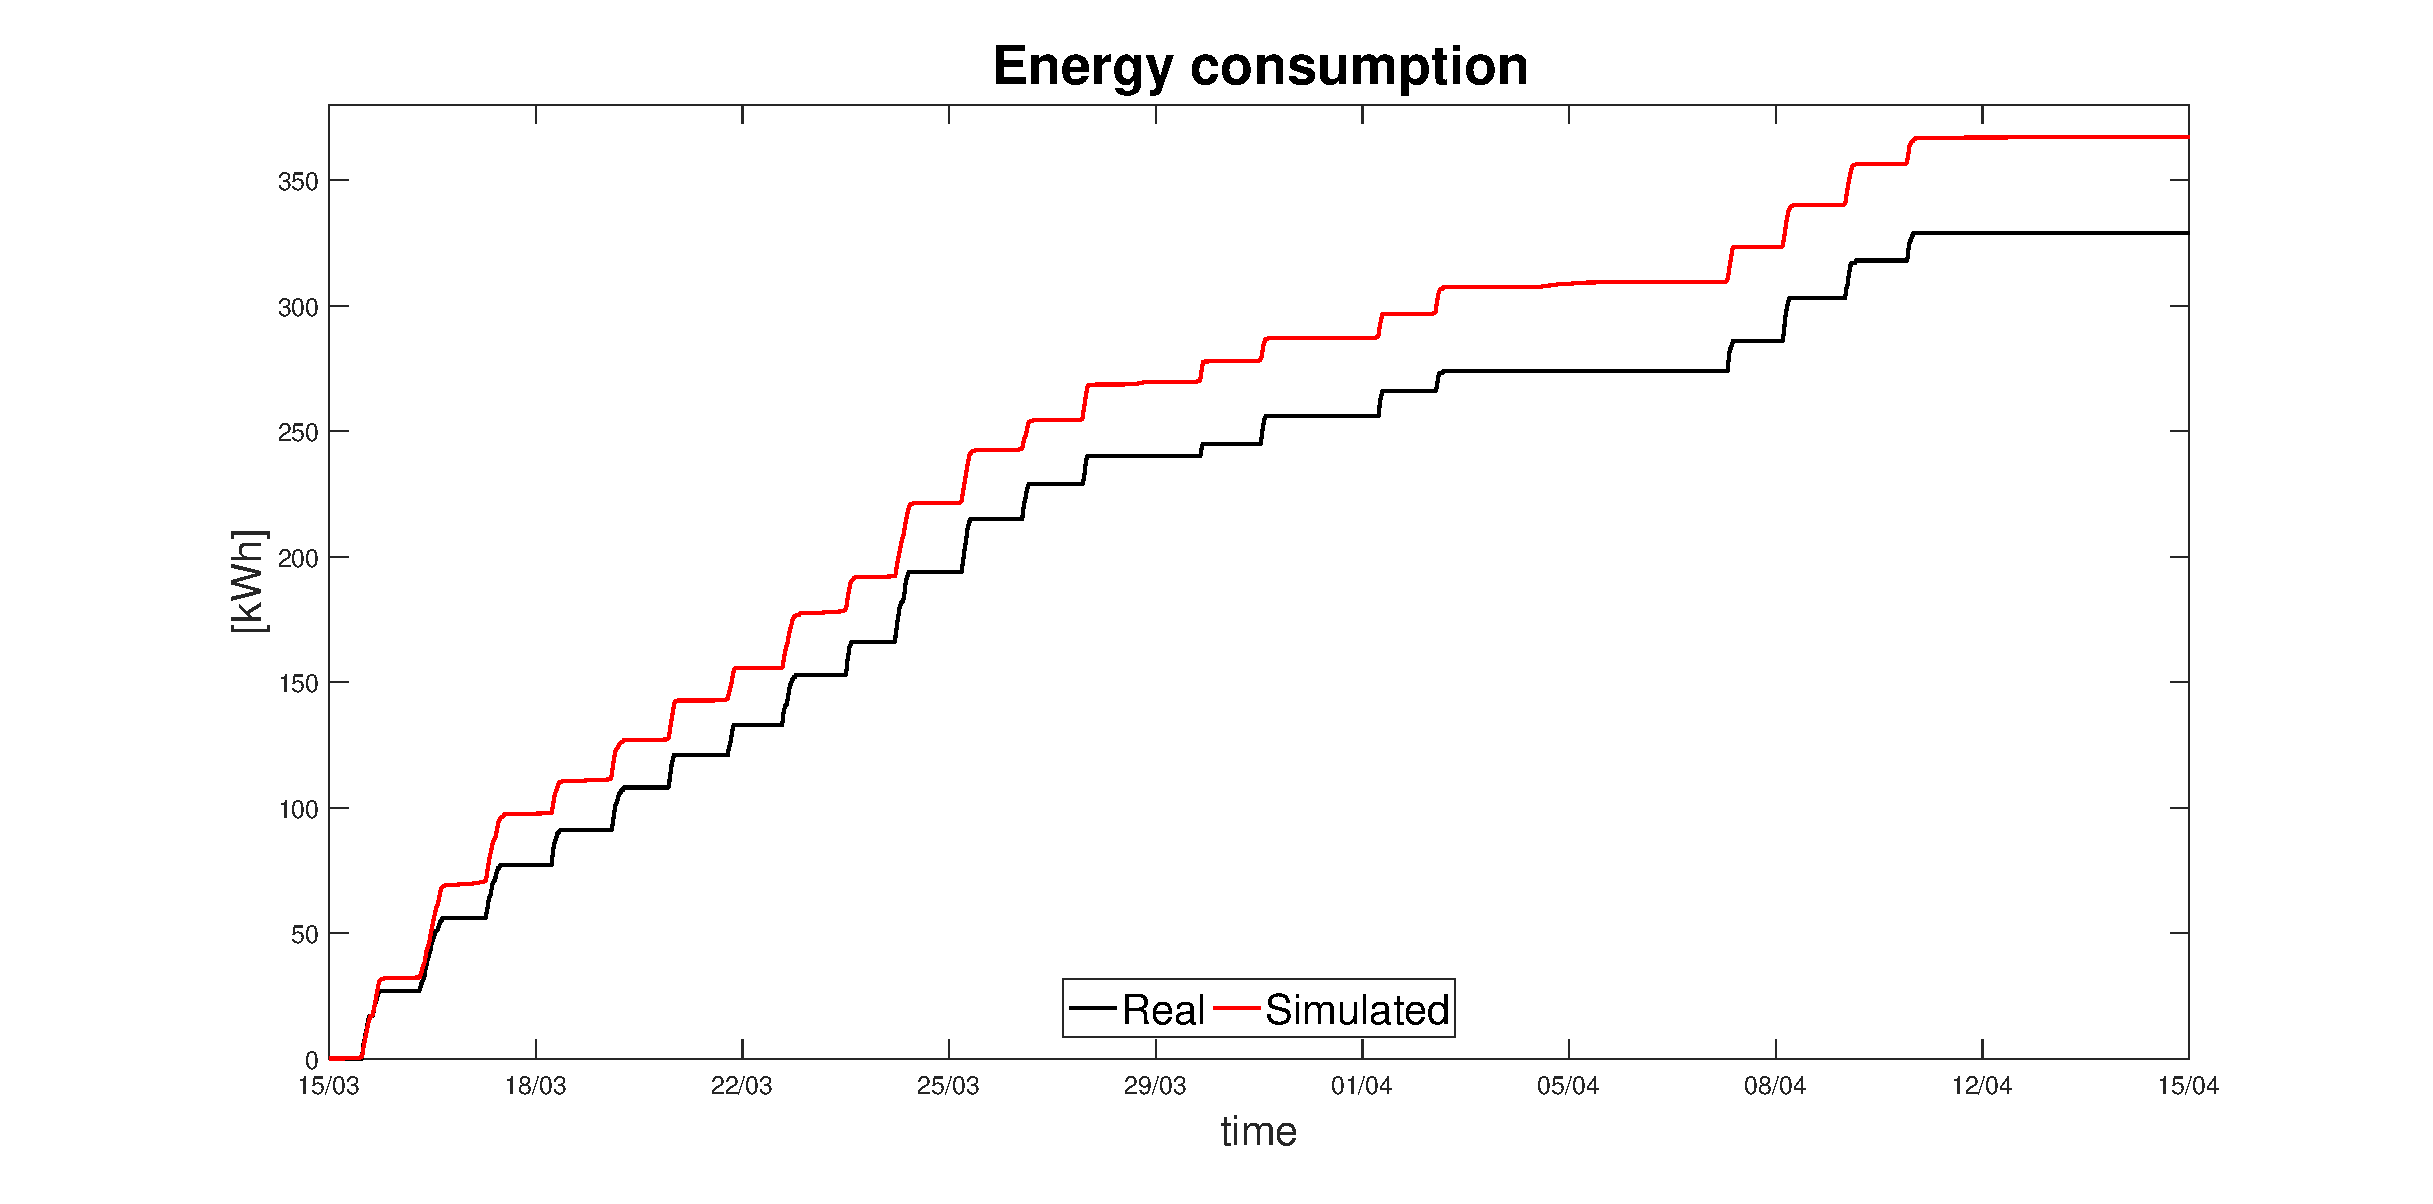
\includegraphics[width=26pc]{figures/Energy_test.eps}
%		\caption{Energy consumption accuracy.}
%		\captionsetup{justification=centering}
%		\label{F:Energy_testing}
%	\end{center}
%\end{figure}
%
%As we can see, with random forest model we get a worse MBE and CV(RMSE) for energy consumption, although the maximum error is very similar. This is because the EnergyPlus model, due to its internal dynamics based on the house structure, is able to compensate the error over time. On the other hand our curve perfectly follows the time behavior of the real case. For this reason, in Section \ref{SS:simulationResults}, we will use both models in order to compare the quality of the DPC with respect to a classical bang-bang controller.

\subsection{DPC and bang-bang controllers}
\label{SS:controllersDPCandBangbang}
We set up $2$ different controllers, DPC and bang-bang controller, to obtain a scheduling policy to switch the radiators ON and OFF in order to keep the temperature of room $3$, i.e. the living room, within a comfort range. Since the heating system serves all of the $4$ rooms simultaneously, without giving the possibility to control the temperature of each room independently, we setup the problem defining the comfort range only for one room. Other rooms temperatures will follow the scheduling policy. Room $3$ has been chosen randomly. In the following we describe the $2$ controllers.

\paragraph{DPC}
We want to optimize the ON/OFF heating system schedule in order to minimize power consumption of the house while keeping temperature of room $3$ within a comfort range. We also allow violations $\epsilon^{min},\epsilon^{max}$  of temperature bounds to guarantee feasibility of the algorithm. We include these violations in the objective function to be minimized.
\begin{table}[t!]
	\centering
	\begin{tabular}{cccccc}
		\toprule
		Set       & Power   & T. room $1$ & T. room $2$ & T. room $3$ & T. room $4$  \\ 
		\midrule
		$S_1$     &         & $96.58$     & $96.99$     & $97.21$     & $96.62$\\
		$S_2$     & $92.21$ & $97.38$     & $97.29$     & $96.93$     & $96.81$\\
		\bottomrule
	\end{tabular}
	\caption{Models accuracy for power and temperatures models in $S_1$ and $S_2$ expressed as $\mathrm{1-NRMSE}\,(\%)$.}
	\captionsetup{justification=centering}
	\label{T:S1accuracy}
	\vspace{-0.5cm}
\end{table}

The problem is set up as follows:

\begin{problem}\label{P:dpcRealCase}
	\begin{align}
		\begin{aligned}
		& \underset{u_{k+j-1},\epsilon_j^{min},\epsilon_j^{max}}{\mathrm{minimize}} & & \sum_{j=1}^{N} Q{\tP}_{k+j}^2 + \lambda_{min}\parallel\epsilon^{min}\parallel_2 + \lambda_{max}\parallel\epsilon^{max}\parallel_2                            \\
		& \mathrm{subject\ to } & & \tP_{k+j}   = \hat{\Theta}_{\tP_j}   [ 1,u_k,\ldots,u_{k+j-1} ]^\top                         \\
		&                    & & \tT^1_{k+j} = \hat{\Theta}_{\tT^1_j} [ 1,u_k,\ldots,u_{k+j-1} ]^\top                            \\
		&                    & & \tT^2_{k+j} = \hat{\Theta}_{\tT^2_j} [ 1,u_k,\ldots,u_{k+j-1} ]^\top                            \\
		&                    & & \tT^3_{k+j} = \hat{\Theta}_{\tT^3_j} [ 1,u_k,\ldots,u_{k+j-1} ]^\top                            \\
		&                    & & \tT^4_{k+j} = \hat{\Theta}_{\tT^4_j} [ 1,u_k,\ldots,u_{k+j-1} ]^\top                            \\
		&                    & & \underline{\tT}_{k+j}-\epsilon^{min}_j\leq\tT^3_{k+j}\leq\overline{\tT}_{k+j}+\epsilon^{max}_j  \\
		&                    & & u_{k+j-1}   = \underline{u} \lor u_{k+j-1} = \overline{u}                                       \\
		&                    & & \epsilon^{min}_j,\epsilon^{max}_j \geq 0, \ j = 1,\dots,N.
		\end{aligned}
	\end{align}\label{E:DPCrealcase}
\end{problem}

\begin{figure}[t!]
	\begin{center}
		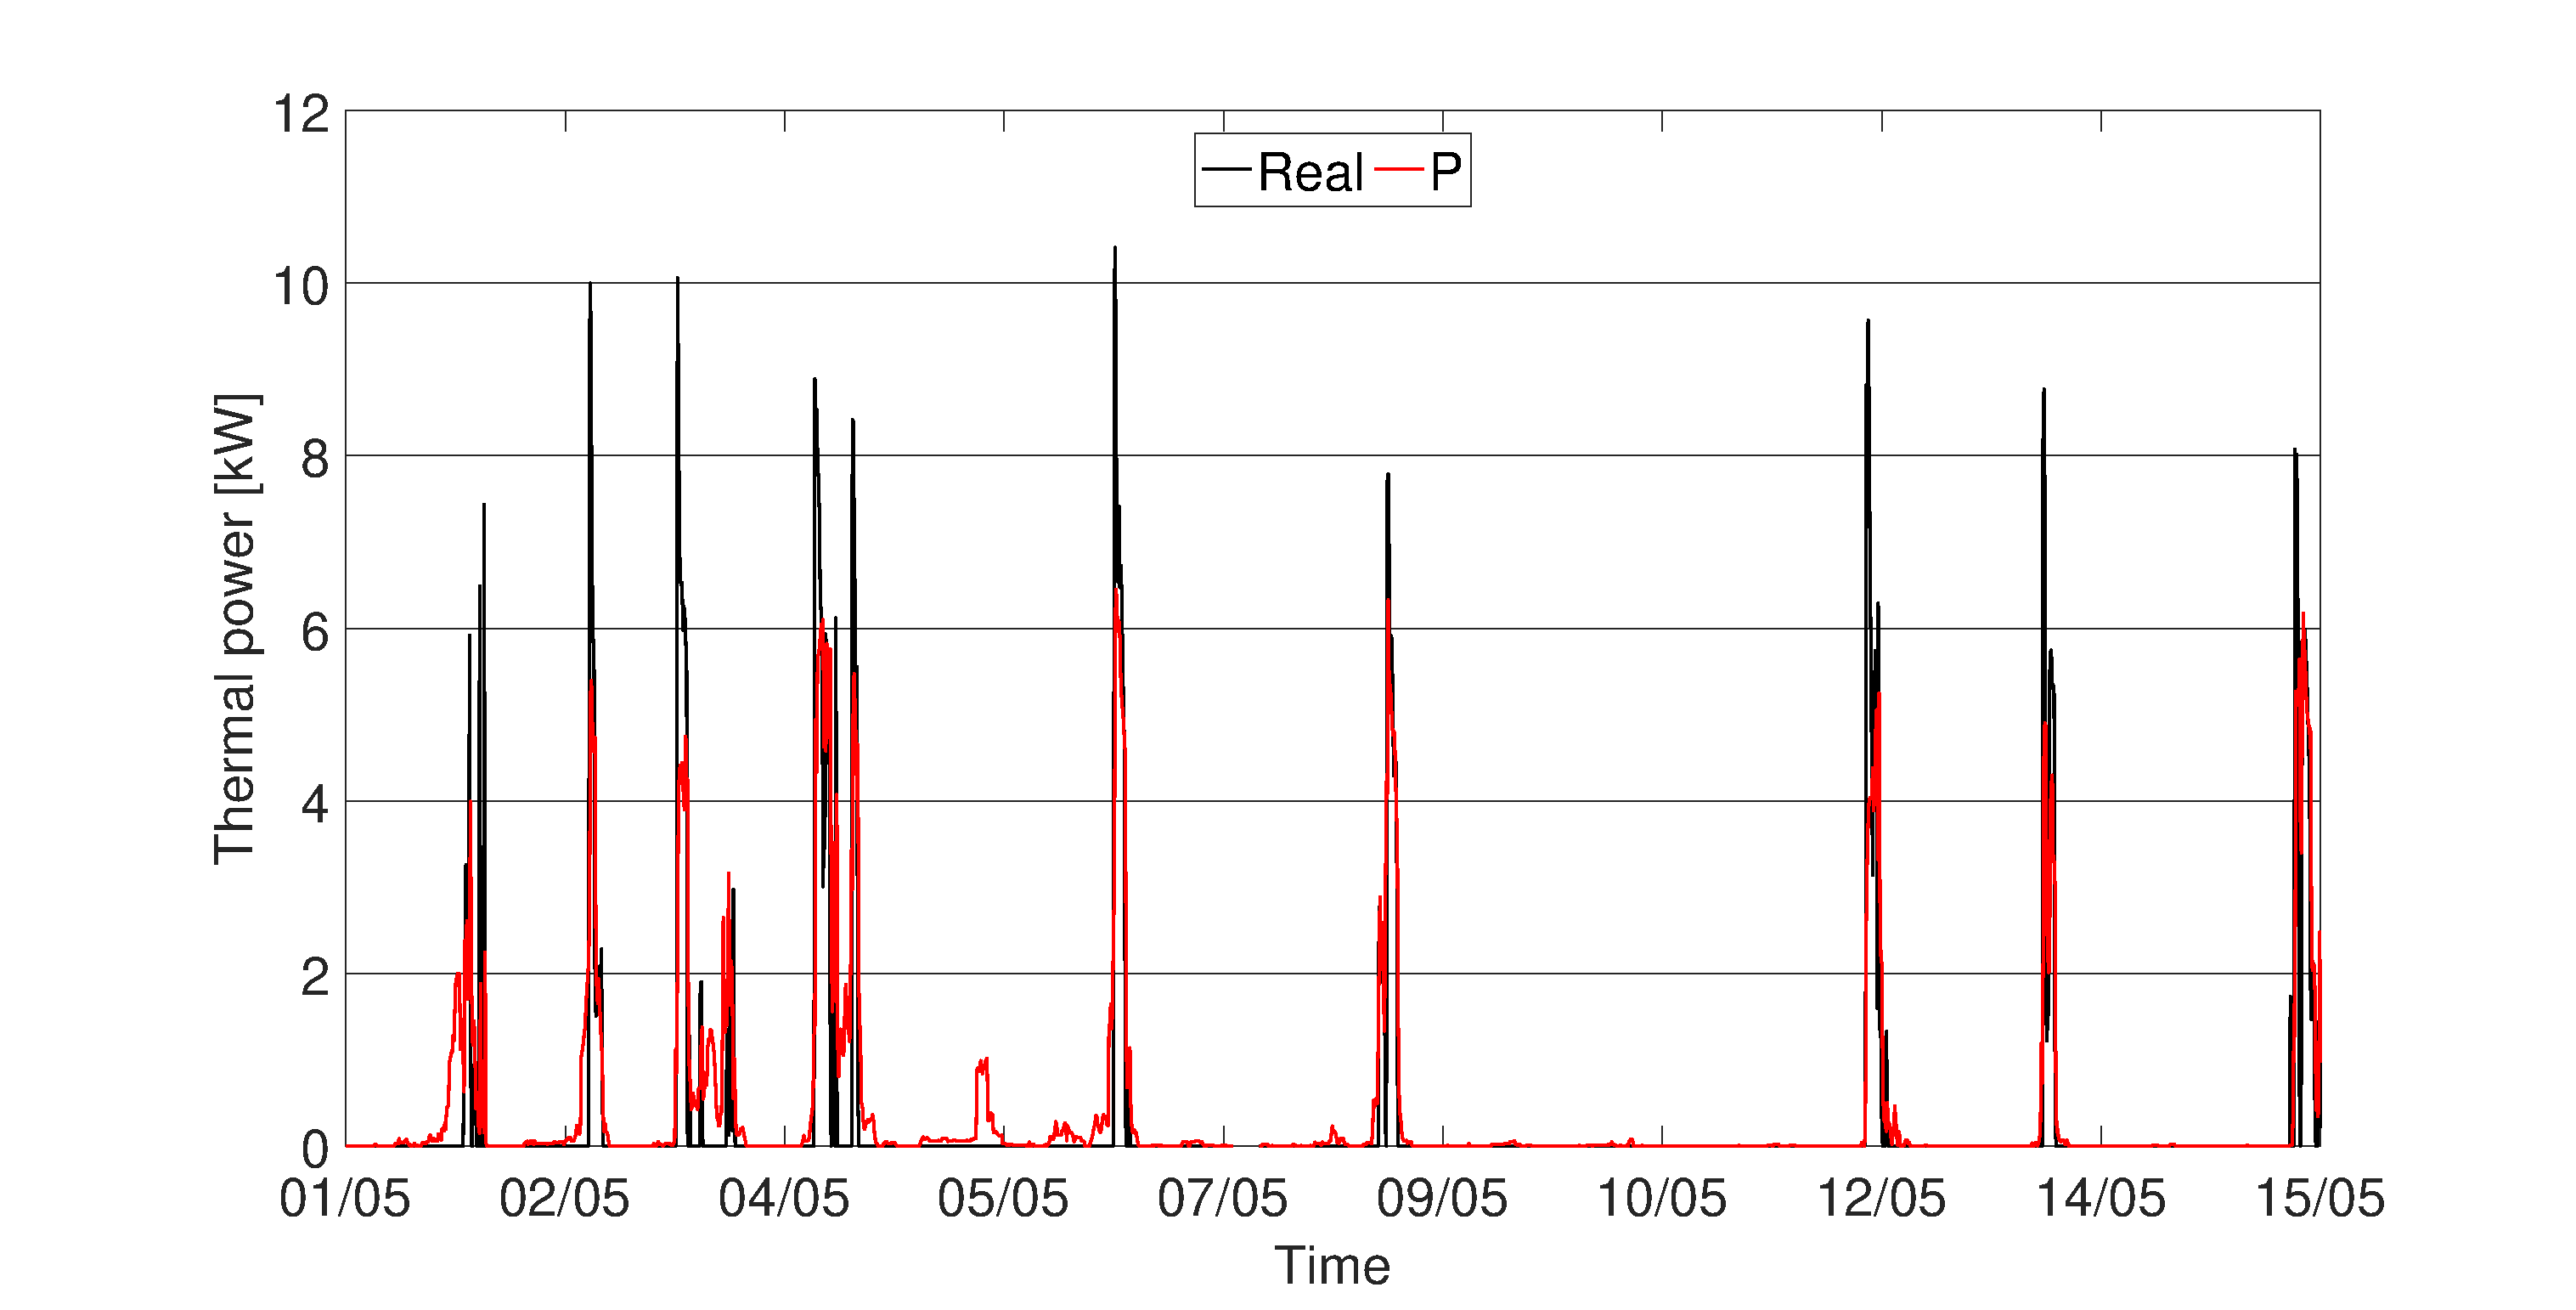
\includegraphics[width=26pc]{figures/power_testing.eps}
		\caption{Power consumption model accuracy validation. The accuracy over the testing period expressed as $\mathrm{1-NRMSE}\,(\%)$ is $92.1\%$.}
		\label{F:power_testing}			
	\end{center}
\end{figure}

\begin{figure}[t!]
	\begin{center}
		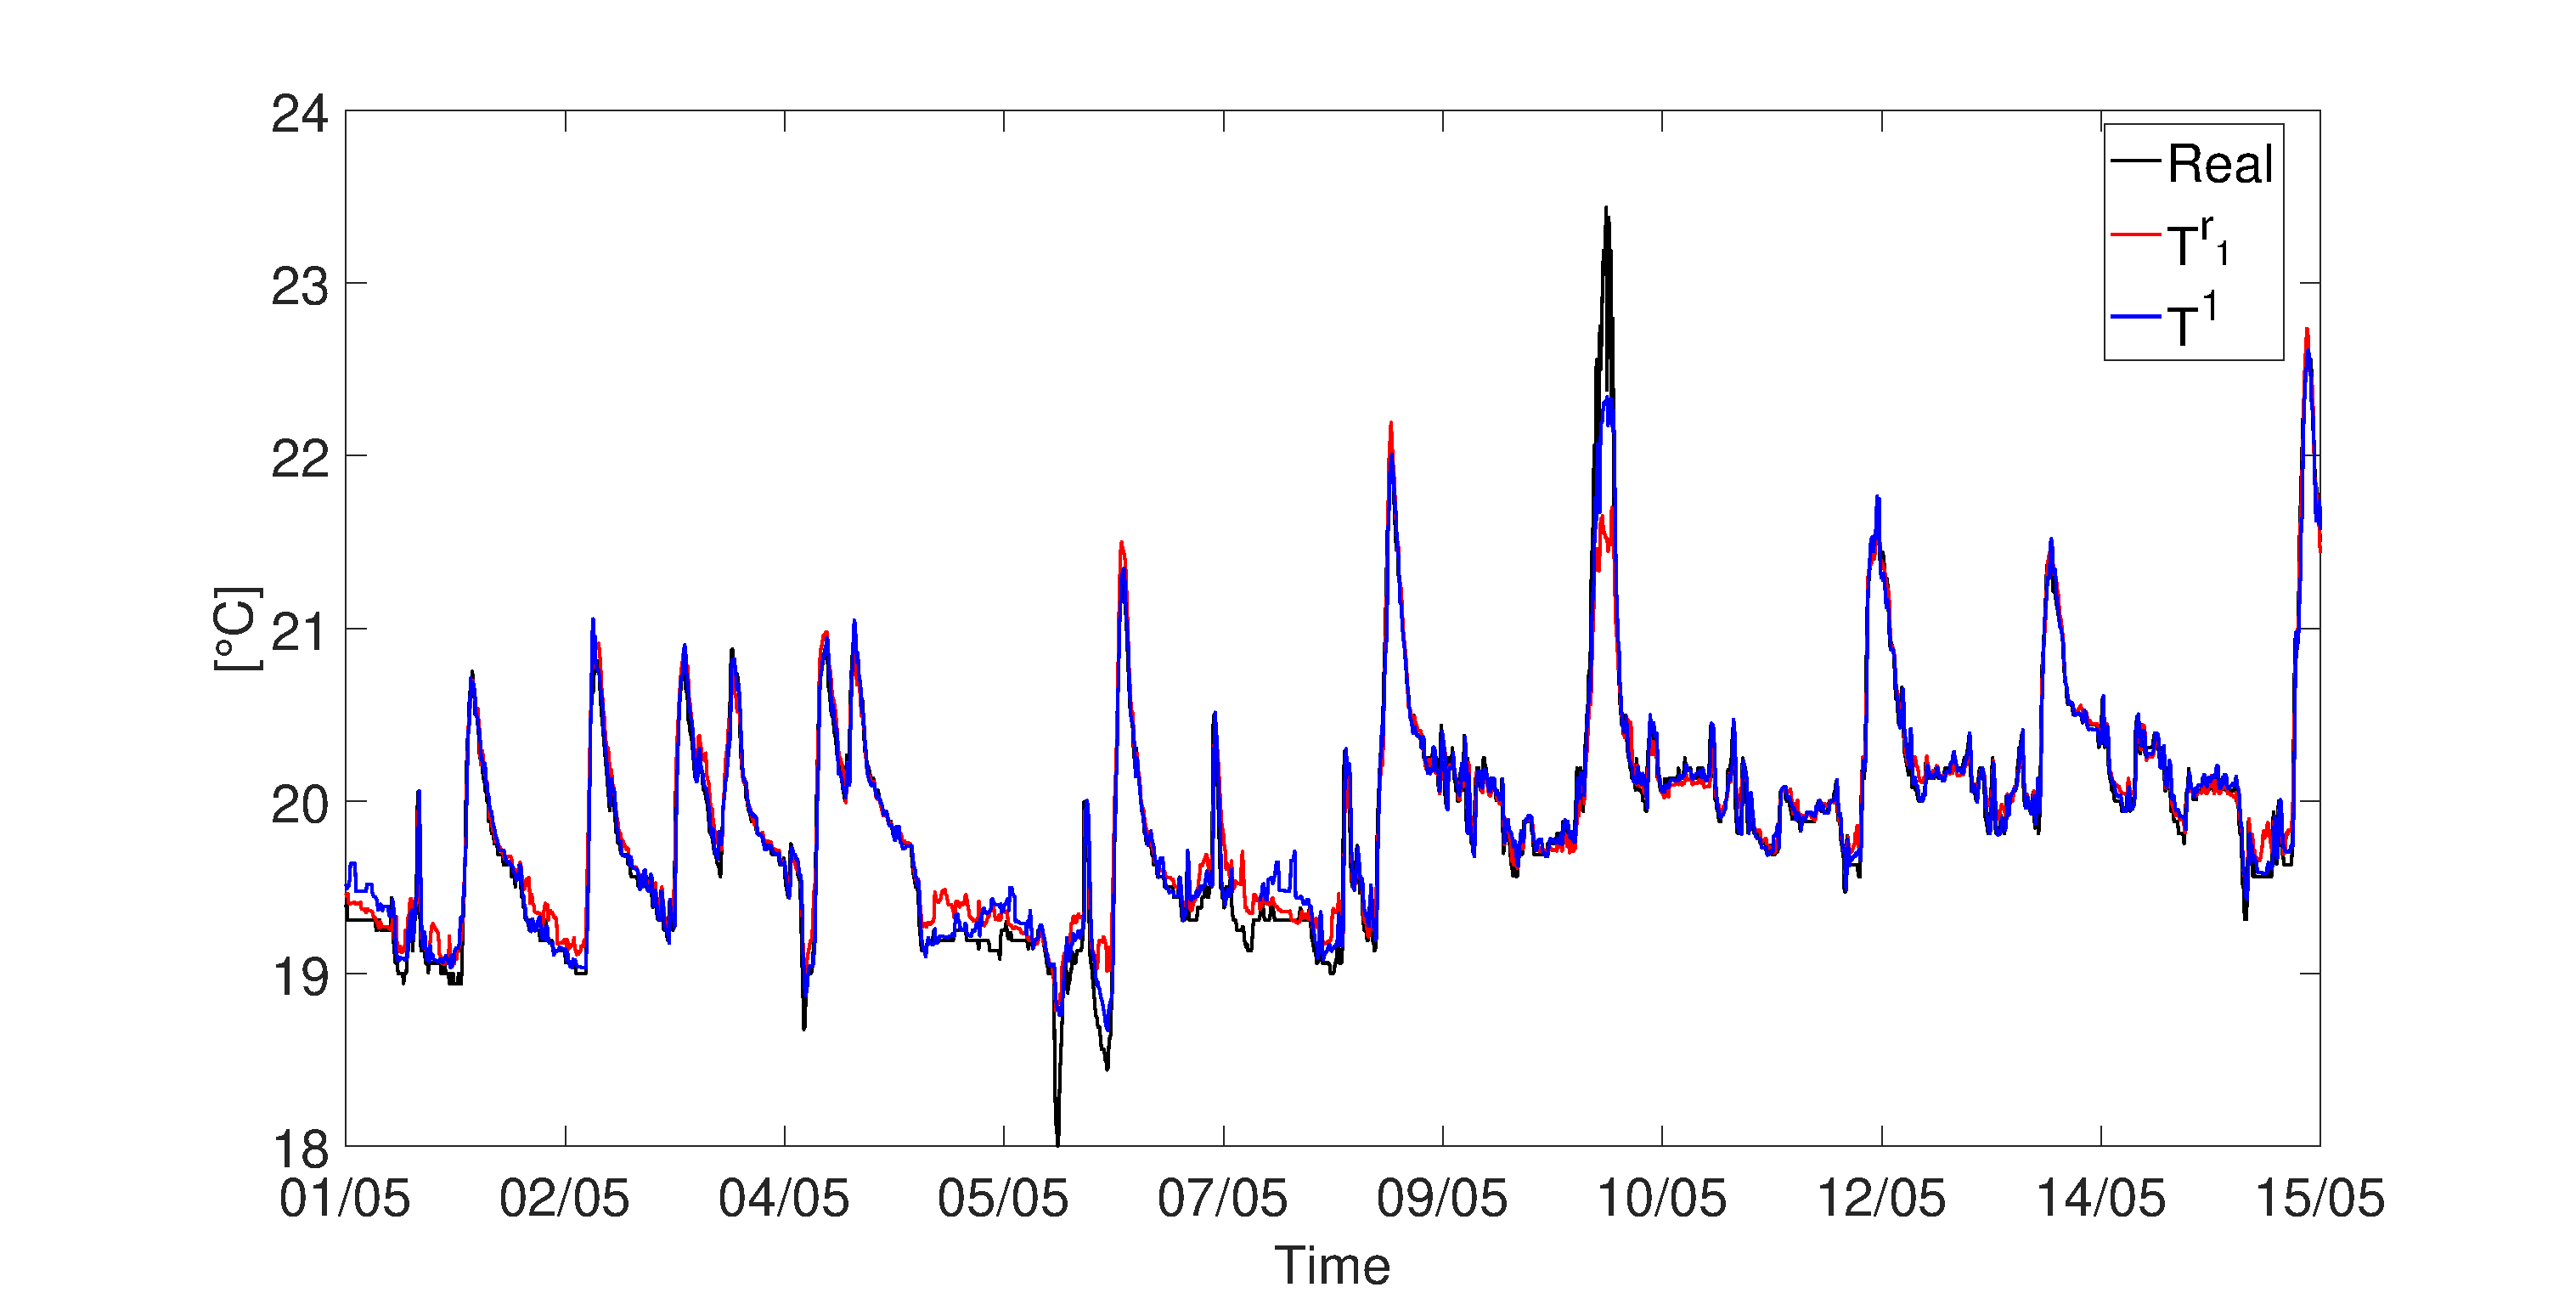
\includegraphics[width=26pc]{figures/temperature_testing.eps}
		\caption{Temperature model accuracy validation for room $1$. The accuracy over the testing period expressed as $\mathrm{1-NRMSE}\,(\%)$ is $96.58\%$, for the temperature model $T^{r_1}$ in $S_1$ and $97.3\%$ for the temperature model $T^1$ in $S_2$. The accuracy for the other rooms is very similar as can be seen in Table \ref{T:S1accuracy}.}
		\label{F:temperature_testing}	
	\end{center}
\end{figure}

The choice of different weights $Q$, $\lambda_{min}$ and $\lambda_{max}$ allows the designer to give more importance to energy consumption rather than temperature comfort and vice versa.
In Section \ref{SS:simulationResults} we will show different performance results considering different weights. Parameters $\underline{u}$ and $\overline{u}$ are respectively minimum and maximum values the heating system can actuate, while $\underline{\tT}_{k+j-1}$ and $\overline{\tT}_{k+j-1}$ are respectively time varying lower and upper bounds to keep the temperature in a desired range of comfort.
Due to the integer variable constraint for input $u$, the problem is a Mixed Integer Quadratic Programming. For the implementation we use in Section \ref{SS:simulationResults} Gurobi solver \cite{Gurobi2015} through CVX \cite{cvx,gb08}.

\paragraph{Bang-bang controller}
This is the classical controller widely used in private houses to keep temperature within a comfort range. It switches the heating system ON when the temperature goes under the temperature lower bound and switches it OFF when the temperature goes over the temperature upper bound. The advantage in using this controller is that it is very simple to set up. On the other hand it uses more energy than actually needed to achieve the task.

\subsection{Simulation Results}\label{SS:simulationResults} We simulated  DPC in \eqref{E:DPCrealcase} and the bang-bang controller, in closed-loop with the house models $\tT^{r_i}_{k+1},\ i=1,\ldots,4$ in $S_1$. We considered a sampling time of $10$ minutes and chose $N=4$ as a predictive horizon, i.e. $40$ minutes. From historical data we got that $\overline{u} = 0.35 \, m^3/h$ when the heating system is ON and obviously $\underline{u} = 0 \, m^3/h$ when the heating system is OFF. For the temperature comfort range we set a constant upper bound $\overline{\tT}_{k} = 22.5 \, \degree C$ and a variable lower bound that is $\underline{\tT}_{k} = 21 \, \degree C$ from $7am$ to $9am$ when people in the house wake up and go out for work, and from $6pm$ to midnight when people come back from work and go to sleep. During other hours when people are either not at home or asleep, we set $\underline{\tT}_{k} = 20 \, \degree C$ 

We explained in Section \ref{SS:descriptionHouse} that the fuel used in the house is vegetable biomass. Therefore, it is not possible to have ON/OFF switching phases too close to each other, differently from a traditional gas boiler, due to the burning process and heat exchange. For this reason we set up both control problems with the constraint that when the heating system is activated it must stay active for at least $20$ minutes. This operating period can be obviously adapted depending on the fuel flow rate.

We ran DPC with $3$ different sets of parameters $Q$, $\lambda_{min}$ and $\lambda_{max}$. Each set allows a different level of temperature bounds violation. In particular, we considered a small ($Q=100$, $\lambda_{min}=3000$ and $\lambda_{max}=100$), a medium ($Q=100$, $\lambda_{min}=1000$ and $\lambda_{max}=100$) and a large ($Q=100$, $\lambda_{min}=100$ and $\lambda_{max}=100$) violation configuration.
\textcolor[rgb]{0,0,1}{The simulation period is of $15$ days, from May $1$, $2016$ at $00am$ to May $15$, $2016$ $00am$.}

\textcolor[rgb]{0,0,1}{We considered 2 different simulative conditions to show the robustness of our approach:
\begin{enumerate}
	\item in Section \ref{SSS:DisturbancePerfect} we provide our simulative results considering perfect knowledge of the weather forecast;
	\item in Section \ref{SSS:DisturbanceUncertain}, we consider weather forecast subject to uncertainty Hence we modify Problem \ref{P:dpcRealCase} by adding a gaussian noise with high variance on the perfect forecast, and show that the results are close to the perfect forecast case, so making our methodology robust with respect to disturbance uncertainties.
\end{enumerate}
\subsubsection{Perfect knowledge of the weather forecast}\label{SSS:DisturbancePerfect}
In this section we ran the simulations considering perfect knowledge of the disturbance over the horizon, obtaining the following results.}
\paragraph{Result 1} The comparison for temperature and input schedule obtained allowing small bound violations in DPC is shown in Figure \ref{F:comparison_small}. For sake of the plot's clarity, the shown period is restricted to $4$ days and a half, from May $1$, $2016$ $00am$ to May $5$, $2016$ $1pm$. \textcolor[rgb]{0,0,1}{The whole period will be used in "Result 2" to provide the bounds violation errors, and in "Result 3" for the energy consumption comparison.}
We can see that the temperature controlled with DPC does not violate the bounds and if it does then the violation is approximately $0.1\,\degree C$. Bang-bang control also presents small bounds violations due to its working principle. We can see how the DPC control law requires the heating system to be ON for less time than the bang-bang one to keep the temperature in the comfort range. 
We will see in Figure \ref{F:comparison_all_energy_E+} that this translates to significant energy saving.

\begin{figure}[t!]
	\begin{center}
	\subfigure[Temperature variation obtained with DPC and bang-bang controller.DPC controller allows almost no violation, so guaranteeing better comfort than bang-bang controller.]{
		\label{F:temperatures_small}
		\centering
		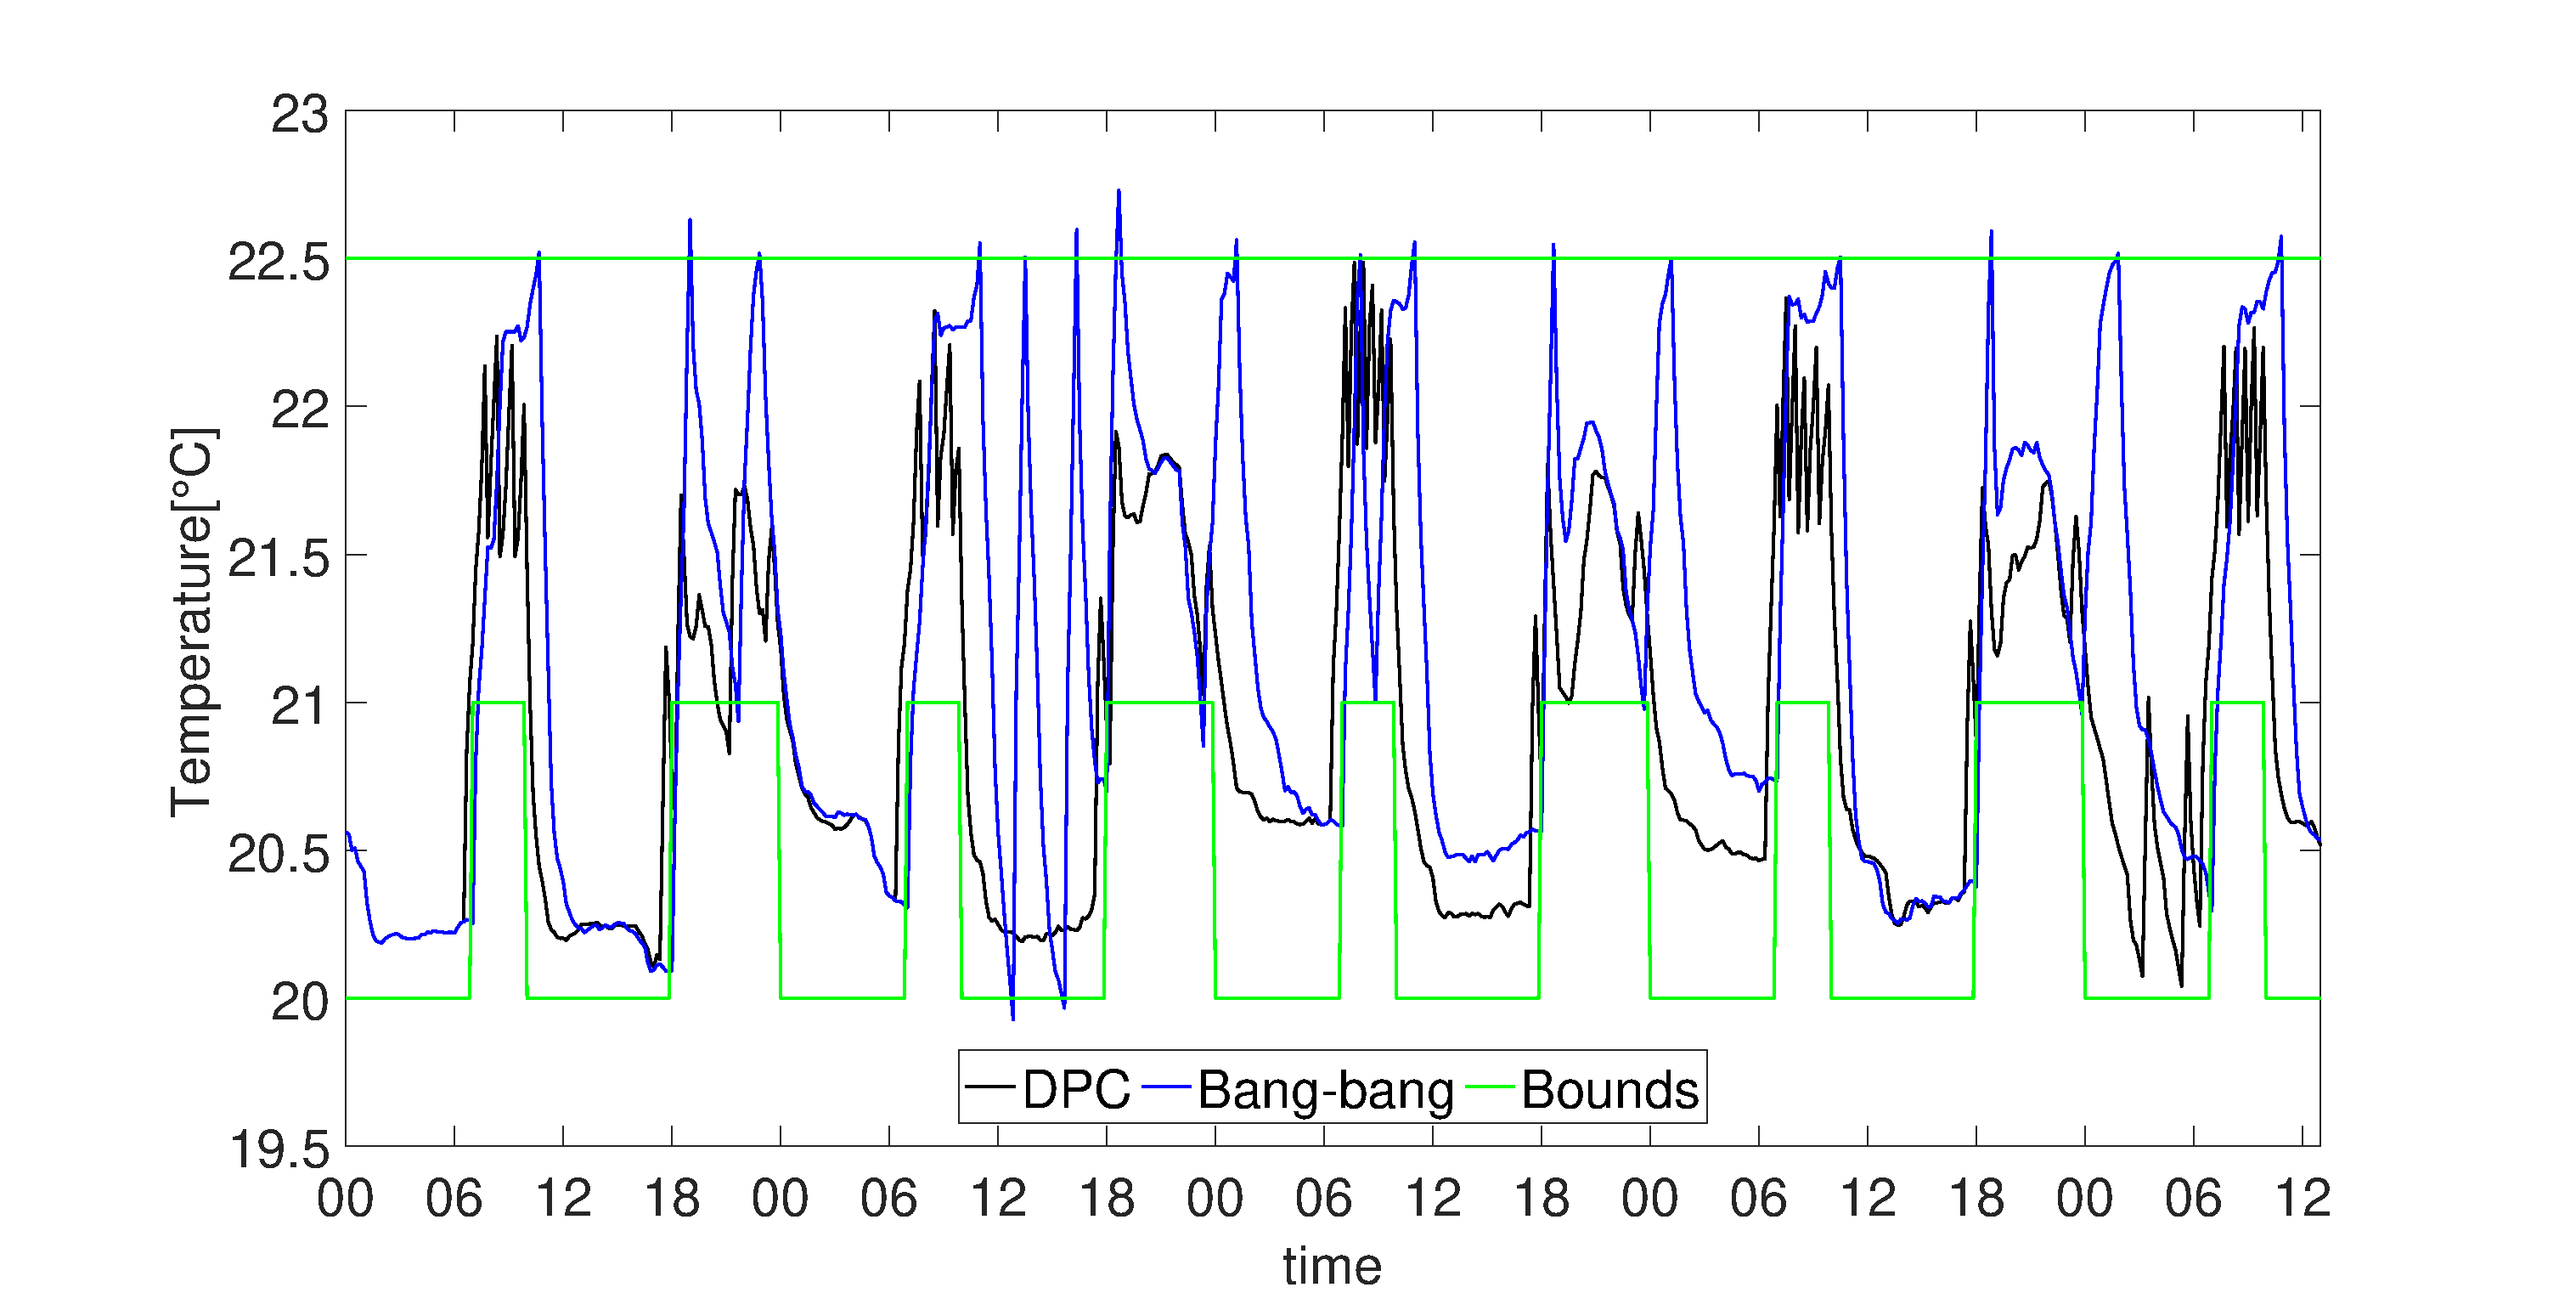
\includegraphics[width=28pc]{figures/Temperatures_small.eps}
	}
	\subfigure[Input schedules obtained from DPC and bang-bang controller. DPC keeps the heating system ON for less time than bang-bang controller, hence saving energy, and guarantees better thermal comfort.]{
		\label{F:inputs_small}
		\centering
		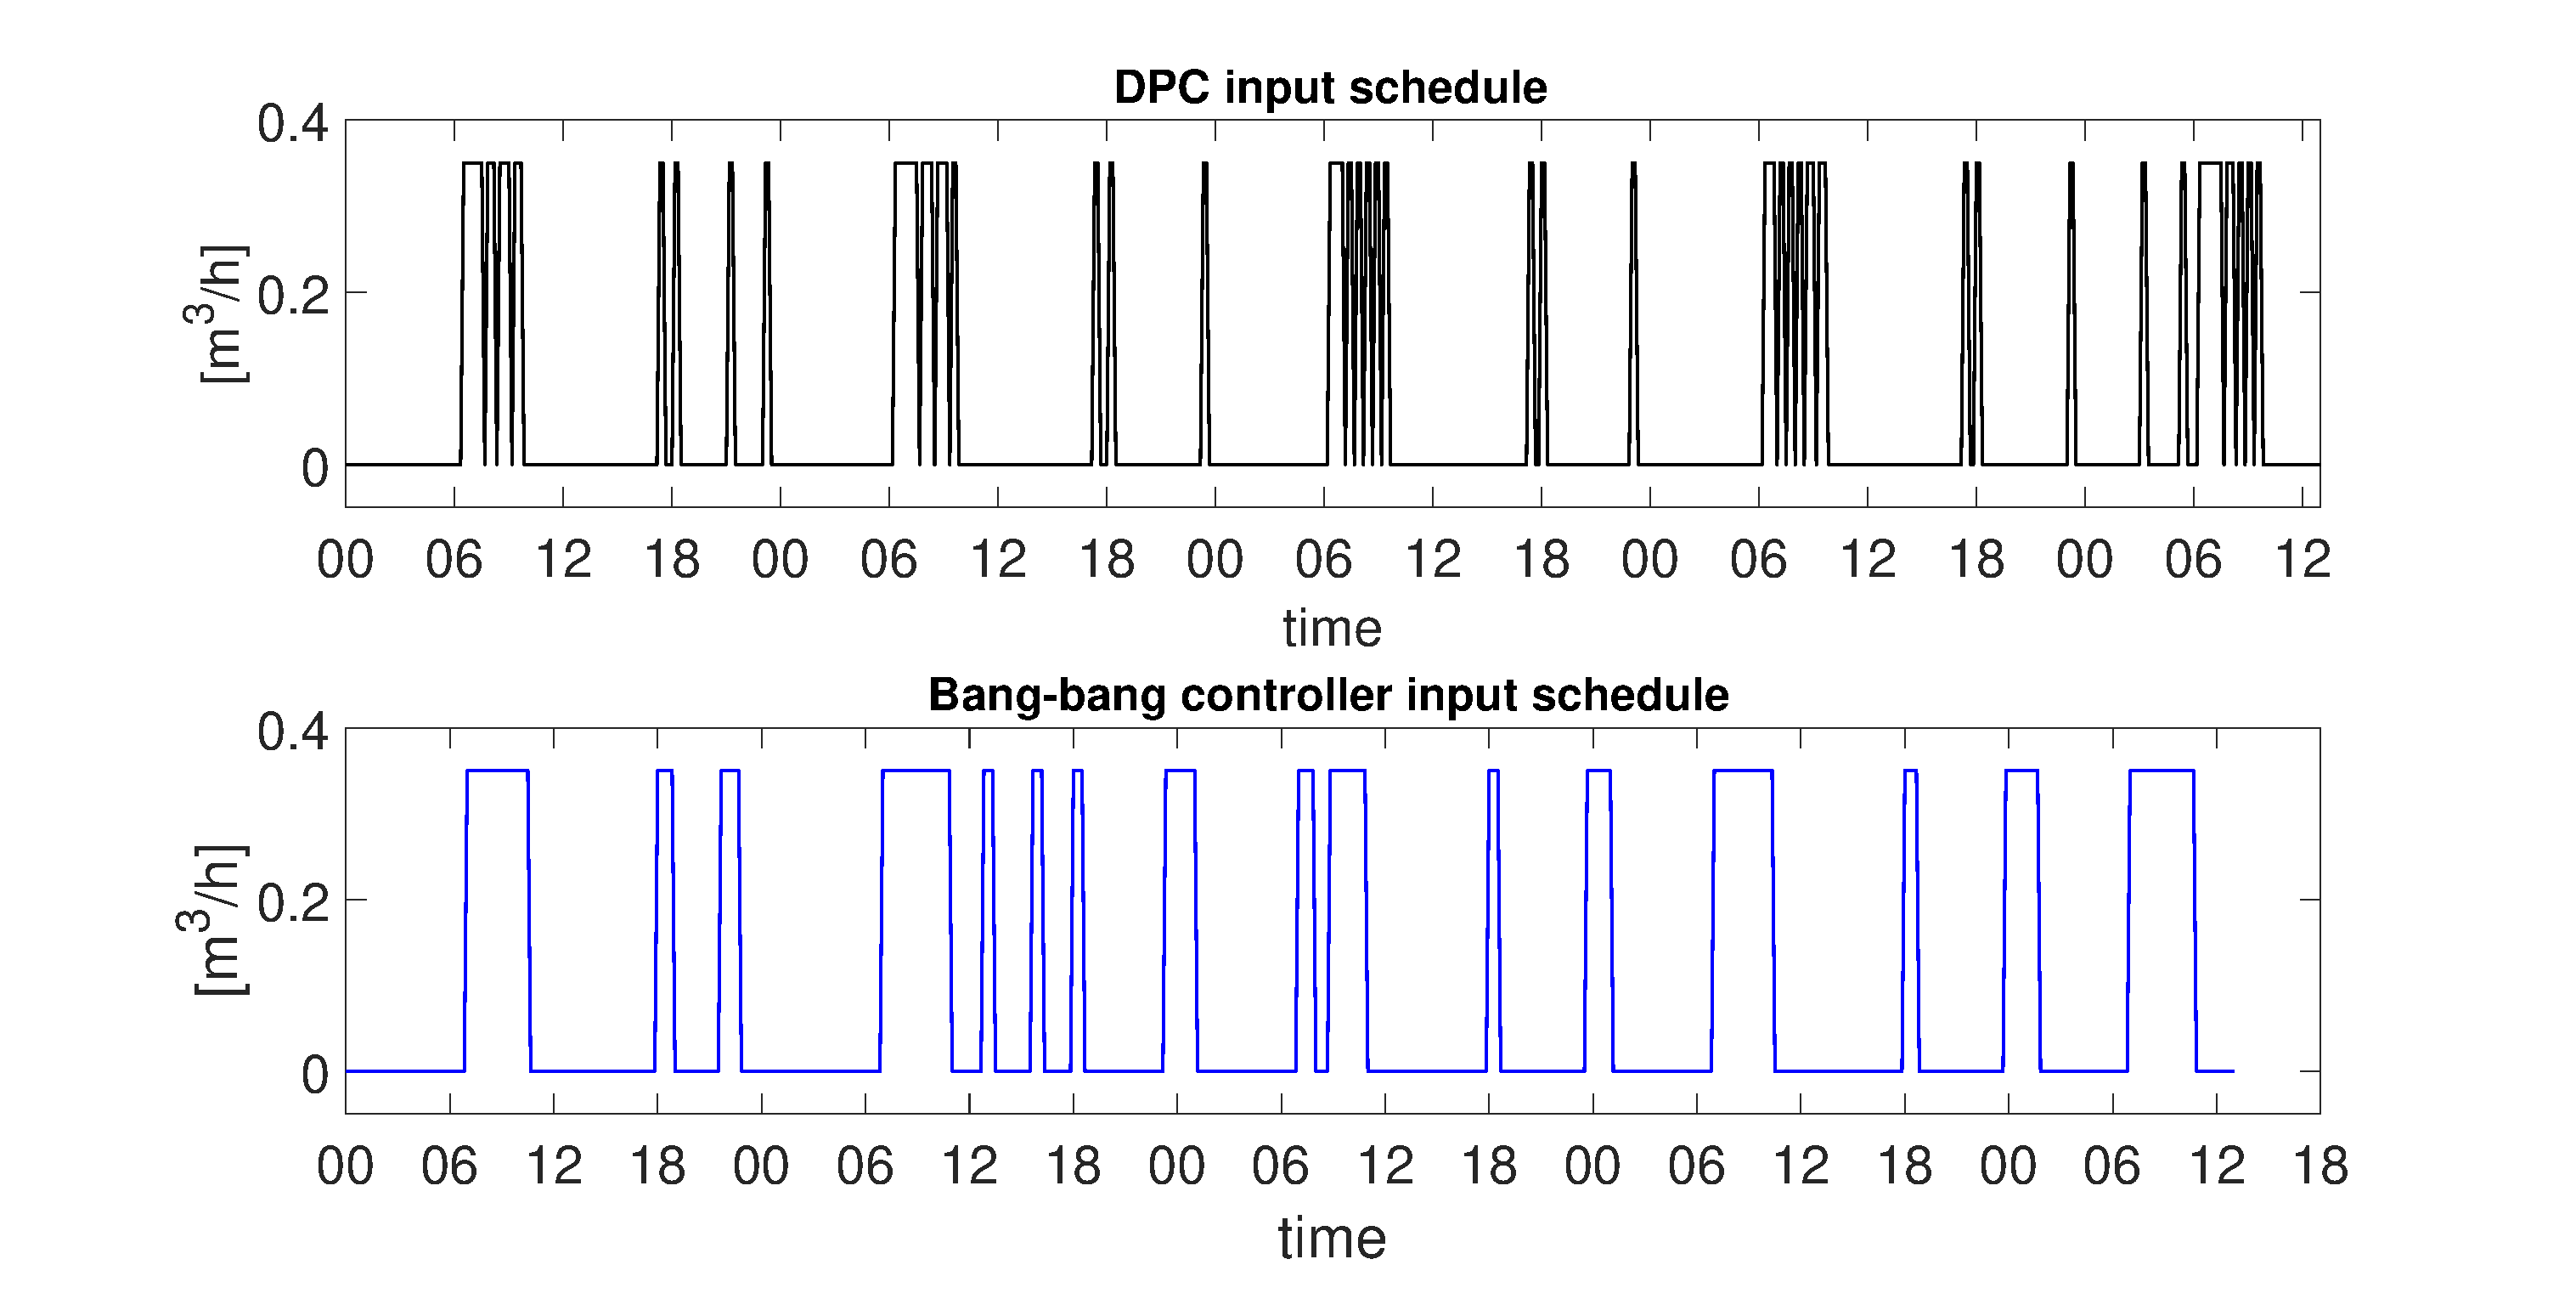
\includegraphics[width=28pc]{figures/Inputs_small.eps}
	}
	\end{center}
\vspace{-0.5cm}
	\caption{Comparison of DPC and bang-bang control performance over $5$ days of the testing period for room $3$.}
	\captionsetup{justification=centering}
	\label{F:comparison_small}
\end{figure}

\paragraph{Result 2} A comparison of temperature regulation obtained running the DPC with small, medium and large violations is shown in Figure \ref{F:comparison_all_temperature}. The results show that with the large violation configuration, that gives more importance to the power consumption minimization than to keep temperature within the bounds, temperature is almost always outside the lower bound during the period when the range is tighter. However the maximum violation is still lower than $1\,\degree C$.
In Table \ref{T:violationErrors}, MBE and CV(RMSE)\textcolor[rgb]{0,0,1}{ (expressed in $\%$, and computed over the whole simulative period, i.e. 15 days) }violation errors are reported to quantify the bounds violation of DPC, in each of the $3$ configurations, and of bang-bang controller. We can see that if we allow very small violations, DPC outperforms bang-bang controller in terms of comfort guarantees.

\paragraph{Result 3} 
%In Figure \ref{F:comparison_all_energy_E+}, using the energy model derived from random forest power model $\tP^r$, we show how DPC outperforms the bang-bang controller also in terms of energy consumption and how the bounds violations allow us to save more energy. We can see that if we want to keep the temperature within a comfort range, only allowing small violations, the use of DPC produce an energy saving of $44\, kWh$, that correspond to the $33.0\%$ over a period of $4$ days and a half. Instead if we allow a large violation over the same period, the energy saving is of $78\, kWh$, that correspond to the $59.0\%$. If we consider these results over a monthly period, i.e. multiplying them for $6$, we get a monthly energy saving that goes from $264\,kWh$ to $468\,kWh$, with different comfort constraint configurations. Considering that the equivalent price of $1\,kWh$ of vegetable biomass is $TOT$\euro{} (TULLIO MAY YOU TELL ME ABOUT THIS PART?), we have a monthly saving of $TOT$\euro{}.

%\begin{figure}[h!]
%	\begin{center}
%		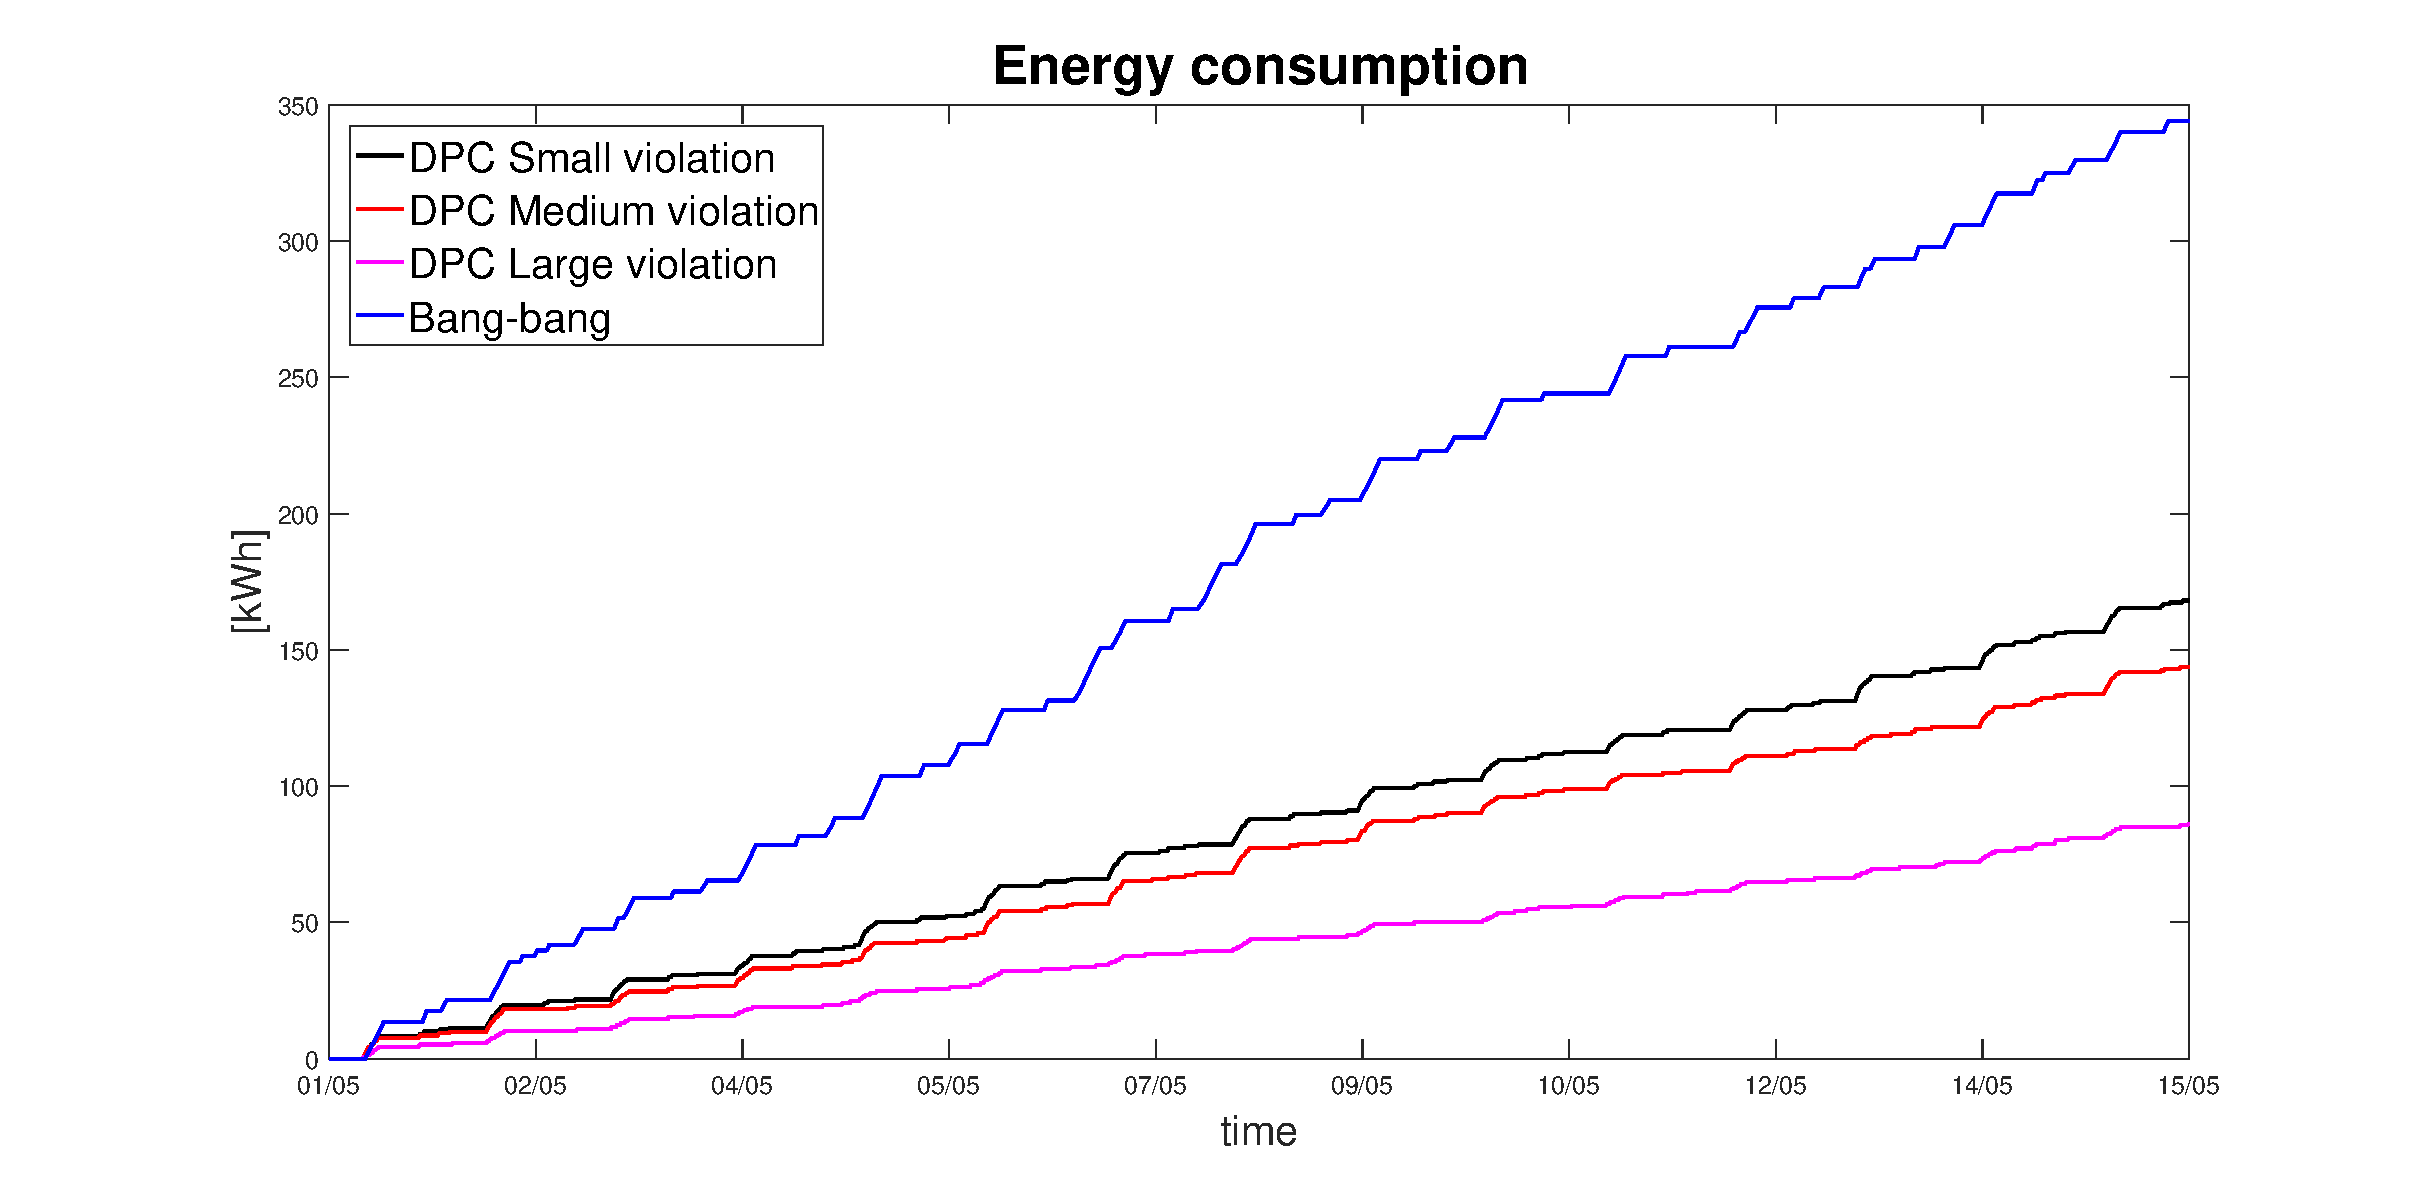
\includegraphics[width=26pc]{figures/Energy_all.eps}
%	\end{center}
%	\caption{Comparison of DPC and bang-bang control performance with different violations using random forest model.}
%	\label{F:comparison_all_energy}
%\end{figure}
%An alternative comparison can be done considering the EnergyPlus model of the house for energy consumption described in Section \ref{SS:energyPlusmodel}. Results are shown in Figure \ref{F:comparison_all_energy_E+}.
In Figure \ref{F:comparison_all_energy_E+}, using the thermal energy consumption model derived in Section \ref{SS:energyPlusmodel} using EnergyPlus, we show how DPC outperforms the bang-bang controller also in terms of energy consumption and how the bounds violations allow us to save more energy. In this case, since the plot is clear and we are interested in showing energy saving on a long period, we ran the simulations over the whole testing period, i.e. $15$ days of May, from May $1$, $2016$ to May $15$, $2016$. We observe that the energy consumption associated to the bang-bang control strategy is approximately equal to $177\,kWh$. If we want to keep the temperature within a comfort range, only allowing small violations, the use of DPC produce an energy saving of $45\, kWh$, that corresponds to the $25.4\%$ over a period of $15$ days. In case of medium violations get an energy saving of $57\, kWh$, that is $32.2\%$. Instead if we allow a large violation over the same period, the energy saving is of $87\, kWh$, that corresponds to the $49.2\%$.
\begin{figure}[t!]
	\begin{center}
		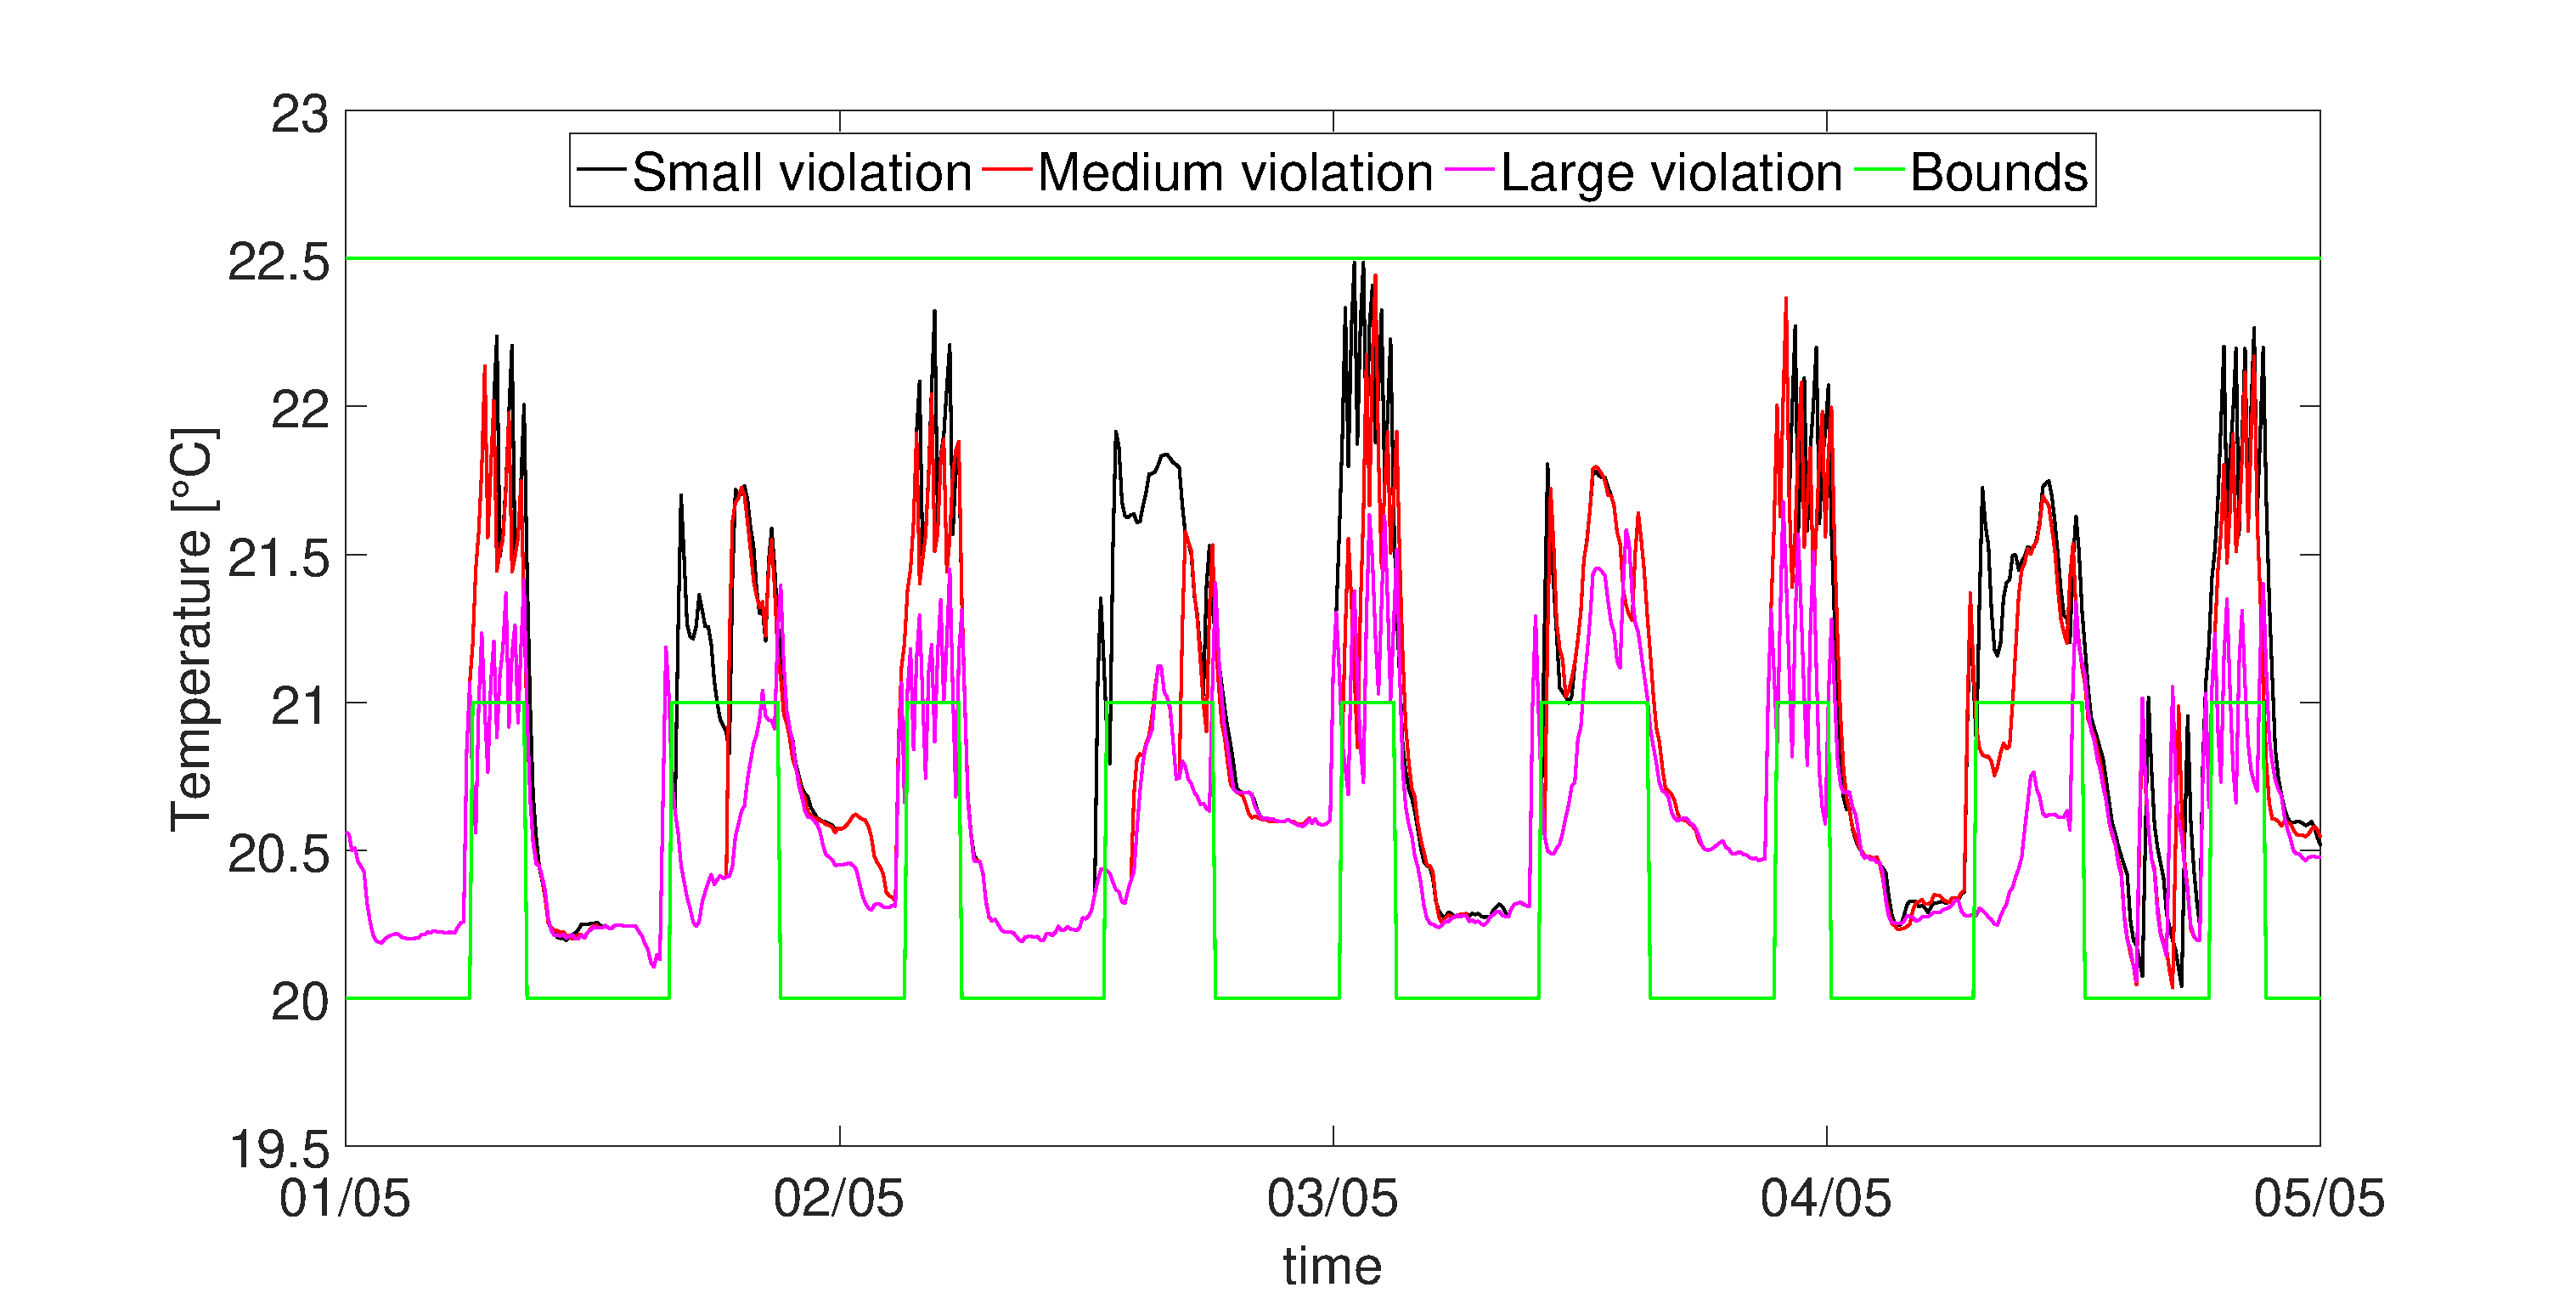
\includegraphics[width=28pc]{figures/Temperatures_all.eps}
	\end{center}
	\caption{Comparison, in terms of comfort, of DPC control performance simulated over $5$ days of the testing period with $3$ different violation configurations: small, medium and large. With the large violation configuration, the temperature is almost always outside of the lower bound when this is tighter. However the maximum bound violation is less than $1\degree C$. With the small violation configuration, the temperature is always within the bound with very few exceptions. However, when it happens, the violation is lower than $0.1\degree C$. The medium violation configuration gives a temperature bound violation that is in the middle with respect to the small and the large ones.}
	\label{F:comparison_all_temperature}
\end{figure}
%\begin{table}[t!]
%	\centering
%	%	\scalebox{0.9}{
%	\begin{tabular}{lccccc}
%		\toprule
%		CONTROLLER  & LBV $\mathrm{MBE}$  & LBV $\mathrm{RMSE}$ & UBV $\mathrm{MBE}$ & UBV $\mathrm{RMSE}$ 	\\ 
%		\midrule
%		$DPC-SV$    & $0.013$             & $0.028$  			      & $0$    				 & $0$     	  	\\
%		$DPC-MV$    & $0.165$ 			  & $0.146$     			  & $0$    				 & $0$		  	\\
%		$DPC-LV$    & $0.410$  			  & $0.224$     			  & $0$    				 & $0$	      	\\
%		$Bang-bang$ & $0.049$ 			  & $0.080$    				  & $0.0063$ 		     & $0.0120$	  	\\
%		\bottomrule
%	\end{tabular}
%	%	}
%	\caption{Lower Bound Violation (LBV) and Upper Bound Violation (UBV) errors expressed as $\mathrm{MBE}\%$ and $\mathrm{CV(RMSE)}\%$ for DPC Small Violation (DPC-SV), DPC Medium Violation (DPC-MV), DPC large Violation (DPC-LV) and bang-bang controller.}
%	\captionsetup{justification=centering}
%	\label{T:violationErrors}
%\end{table}
\begin{table}[t!]
	\centering
	%	\scalebox{0.9}{
	\begin{tabular}{lccccc}
		\toprule
		CONTROLLER  & LBV $\mathrm{MBE}$  & LBV $\mathrm{RMSE}$ & UBV $\mathrm{MBE}$ & UBV $\mathrm{RMSE}$ 	\\ 
		\midrule
		$DPC-SV$    & $0.013$             & $0.092$  			      & $0$    				 & $0$     	  	\\
		$DPC-MV$    & $0.165$ 			  & $0.479$     			  & $0$    				 & $0$		  	\\
		$DPC-LV$    & $0.410$  			  & $0.733$     			  & $0$    				 & $0$	      	\\
		$Bang-bang$ & $0.0485$ 			  & $0.265$    				  & $0.0063$ 		     & $0.040$	  	\\
		\bottomrule
	\end{tabular}
	%	}
	\caption{Lower Bound Violation (LBV) and Upper Bound Violation (UBV) errors expressed as $\mathrm{MBE}\%$ and $\mathrm{CV(RMSE)}\%$ for DPC Small Violation (DPC-SV), DPC Medium Violation (DPC-MV), DPC large Violation (DPC-LV) and bang-bang controller.}
	\captionsetup{justification=centering}
	\label{T:violationErrors}
\end{table}
\begin{figure}[t!]
	\begin{center}
		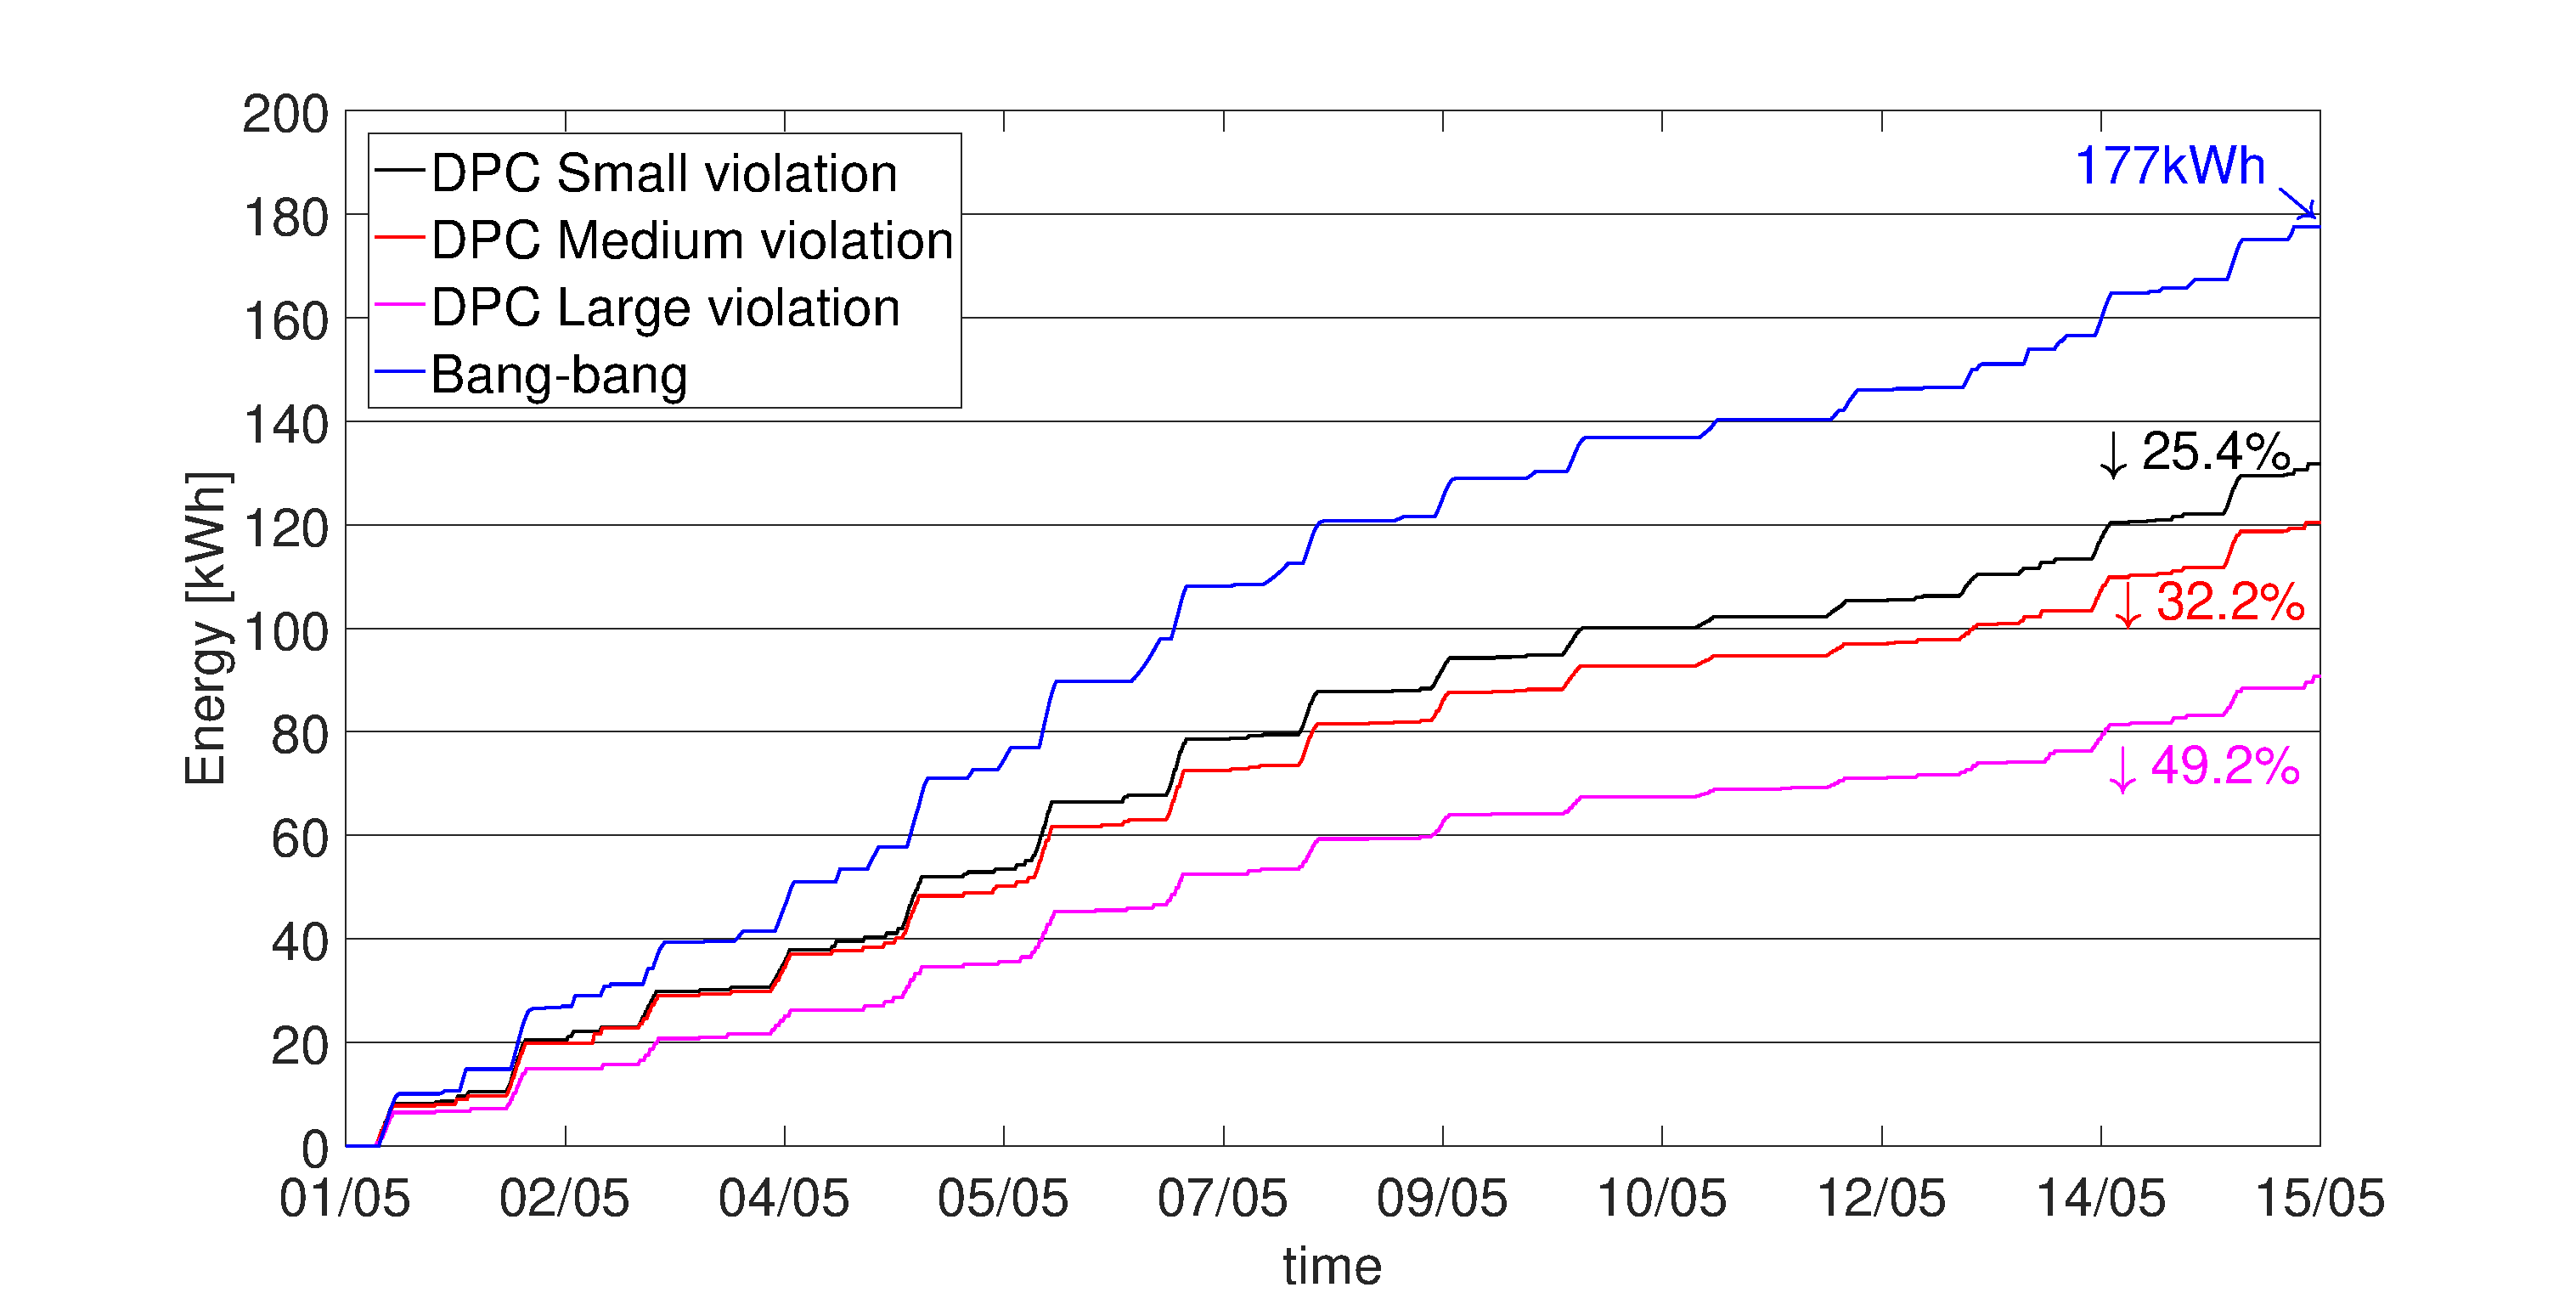
\includegraphics[width=28pc]{figures/Energy_all_EnergyPlus.eps}
	\end{center}
	\caption{Comparison of DPC and bang-bang controller performance over $15$ days of the testing period with different violation configurations, in terms of thermal energy saving using EnergyPlus model. Using bang-bang controller the house energy consumption after $15$ days is of $177kWh$. DPC with small, medium and large violation configurations allows an energy saving of $25.4\%$, $32.3\%$ and $49.2\%$ respectively.}
	\label{F:comparison_all_energy_E+}
\end{figure}

\textcolor[rgb]{0,0,1}{
\subsubsection{Weather forecast subject to uncertainty}\label{SSS:DisturbanceUncertain}
In \cite{Petersen2014AE} the authors investigated, through a large-scale simulation study, the effect of weather forecast uncertainty on the performance of MPC in building systems operations, and compared to the performance of a rule-based strategy.
They considered 48 different scenarios of uncertainties on 72 hours weather forecast.
On such long horizon, results have shown that, with few exceptions, MPC outperforms the rule-based controller in case of energy savings and/or thermal indoor environment, and is in general quite close to the perfect forecast case, despite the uncertainty in weather forecast.}

\textcolor[rgb]{0,0,1}{Horizon length for the DPC algorithm presented in this paper is usually much shorter, as for example $6\ hours$ in Section \ref{S:proof}, $7\ hours$ in Section \ref{S:casestudy}, and $40\ minutes$ in Section \ref{S:realCaseStudy}. This means the weather forecast is more accurate than the 72 hours case presented in \cite{Petersen2014AE}, hence also control performance is even closer to the perfect knowledge forecast case.
Nevertheless, to show the robustness of our approach, in this section we provide simulations considering noisy weather forecast.}

\textcolor[rgb]{0,0,1}{To this aim, we add noises with normal distribution on the disturbance variables in $\X^d$, used to obtain parameters $\hat \Theta$ in the DPC problem \eqref{E:DPCrealcase}, i.e. the disturbance in input in the blue rectangle in Figure \ref{F:overview}, while we use the correct ones to simulate the process, i.e. the disturbance in input in the "Plant" box in the red rectangle in Figure \ref{F:overview}.
In Table \ref{T:NoiseParameters} we summarize the mean and the deviation values of the Gaussian noises that we add to each variable.
We obviously do not add any noise on the "Time of the day" and on the "Day of the week" since those are perfectly known.
We considered zero mean since we suppose there is no constant offset in the forecast, but only an error that can over or underestimate the predictions.
In the table, we also report the range of the values that the variables assumed during the reference period of the historical dataset.
This is to show that the deviation values we chose add a quite bad error on the forecast.
In particular, for example, a deviation of $0.5\degree C$ on the outside air temperature means that the error on the predicted temperature lies within the range of $\pm 1.5\degree C$ with a probability of $99\%$.
We solved DPC problem \ref{P:dpcRealCase} considering the new parameters $\hat \Theta$, obtained using the aforementioned noisy forecast, obtaining the following results, where we show the change in performance on bounds violation and energy consumption due to the forecast inaccuracy.}
\begin{table}[t!]
	\centering	
	\textcolor[rgb]{0,0,1}{\begin{tabular}{lccc}
		\toprule
		Variable               & Range      & Mean & Deviation \\ 
		\midrule
		Outside temperature    & [0,31]     & 0	   & 0.5       \\
		Wind                   & [0,5] 		& 0    & 0.25      \\
		Atmospheric pressure   & [990,1030] & 0    & 50        \\
		Relative Humidity      & [20,91]	& 0    & 5         \\
		Solar Radiation        & [0,1000]   & 0    & 50        \\
		Time of the day        & [0,23]     & 0    & 0         \\
		Day of the week        & [1,7]      & 0    & 0         \\
		\bottomrule
	\end{tabular}}
	\caption{\textcolor[rgb]{0,0,1}{Mean and deviation values of the Gaussian noises added on the weather forecast data, and the range of variation of the variables in the historical dataset.}}
	\captionsetup{justification=centering}
	\label{T:NoiseParameters}
\end{table}

\textcolor[rgb]{0,0,1}{\paragraph{Result 1} In Figure \ref{F:ComparisonTempNoisy} a comparison of the DPC results in terms of temperature control for thermal comfort, between the perfect and the noisy forecast, is shown.
Also here, for the sake of plot's clarity, we show only 4 days and a half of the 15 days simulative period, and we split the plot into 3 sub-figures referring to the small, medium and large violation cases.
We can see that, except for an isolated case in the medium violation case (slightly before the "02/05"), we have a small performance deterioration in terms of bounds violation, although this is more highlighted in the large violation case.
However, the maximum violation, as in the case of perfect forecast, is still lower than $1\,\degree C$.
In particular, we report in Table \ref{T:violationErrorsNoisy} the violation errors in terms of MBE and CV(RMSE) (in $\%$) computed for the whole simulative period, i.e. 15 days.
If we compare them with the ones in Table \ref{T:violationErrors}, we can see that the performance of DPC with noisy forecast are still good with respect to the performance of DPC with perfect forecast, despite the extremely bad prediction error that we considered on the weather forecast.
}
\begin{figure}[t!]
	\begin{center}
		\vspace{1.1cm}
		\subfigure{
			\label{F:SmallNoisy}
			\centering
			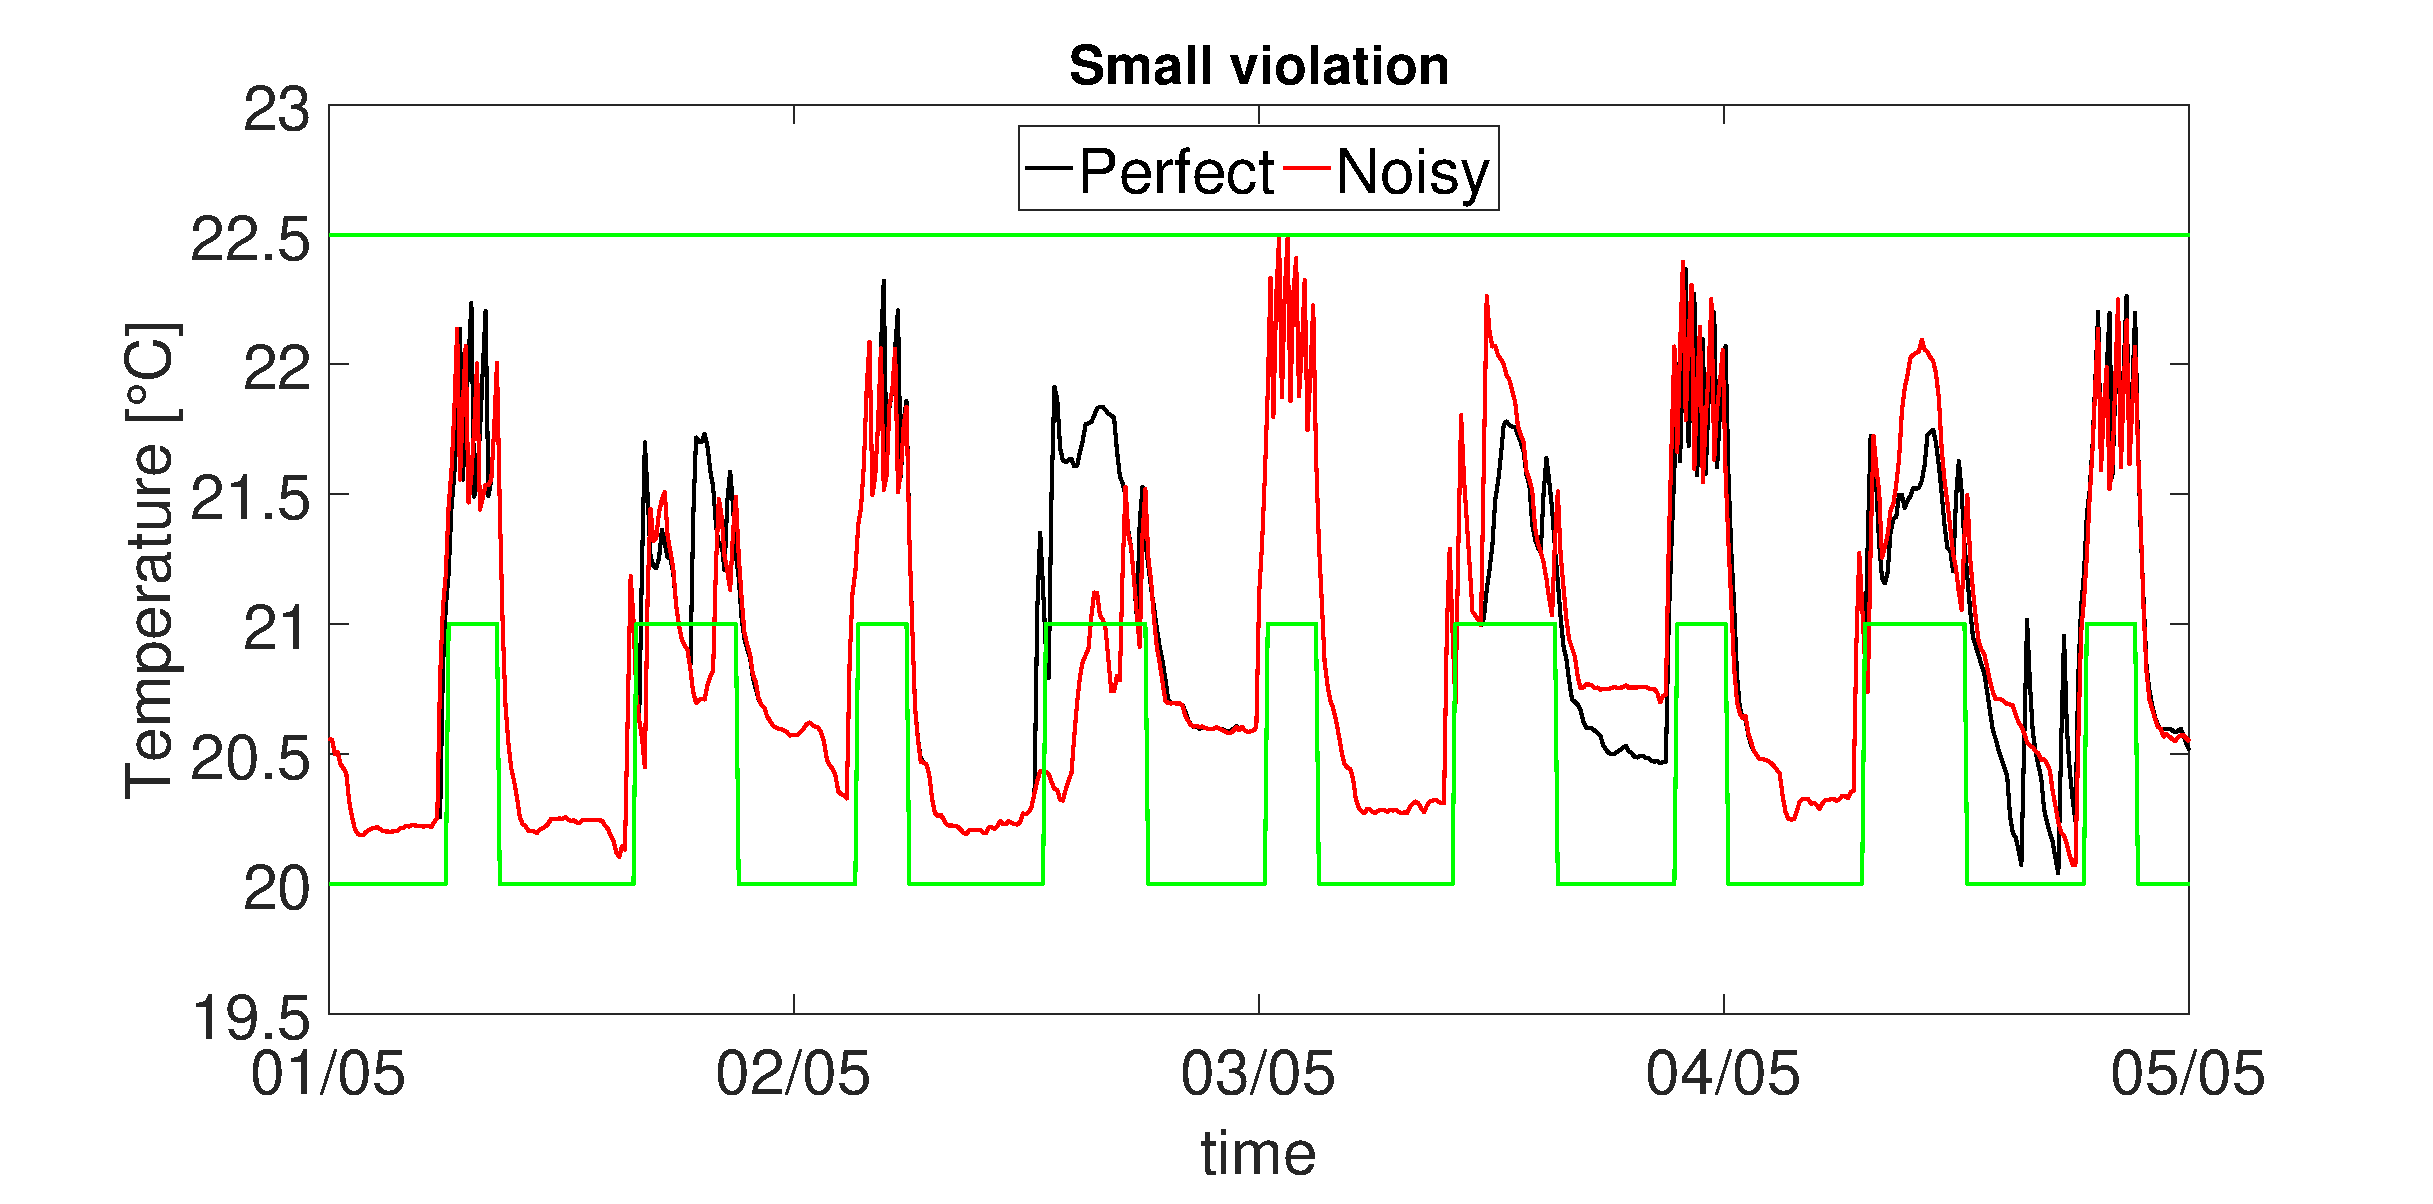
\includegraphics[width=23pc]{figures/Temperatures_small_noisy.eps}
		}	
		\subfigure{
			\label{F:MediumNoisy}
			\centering
			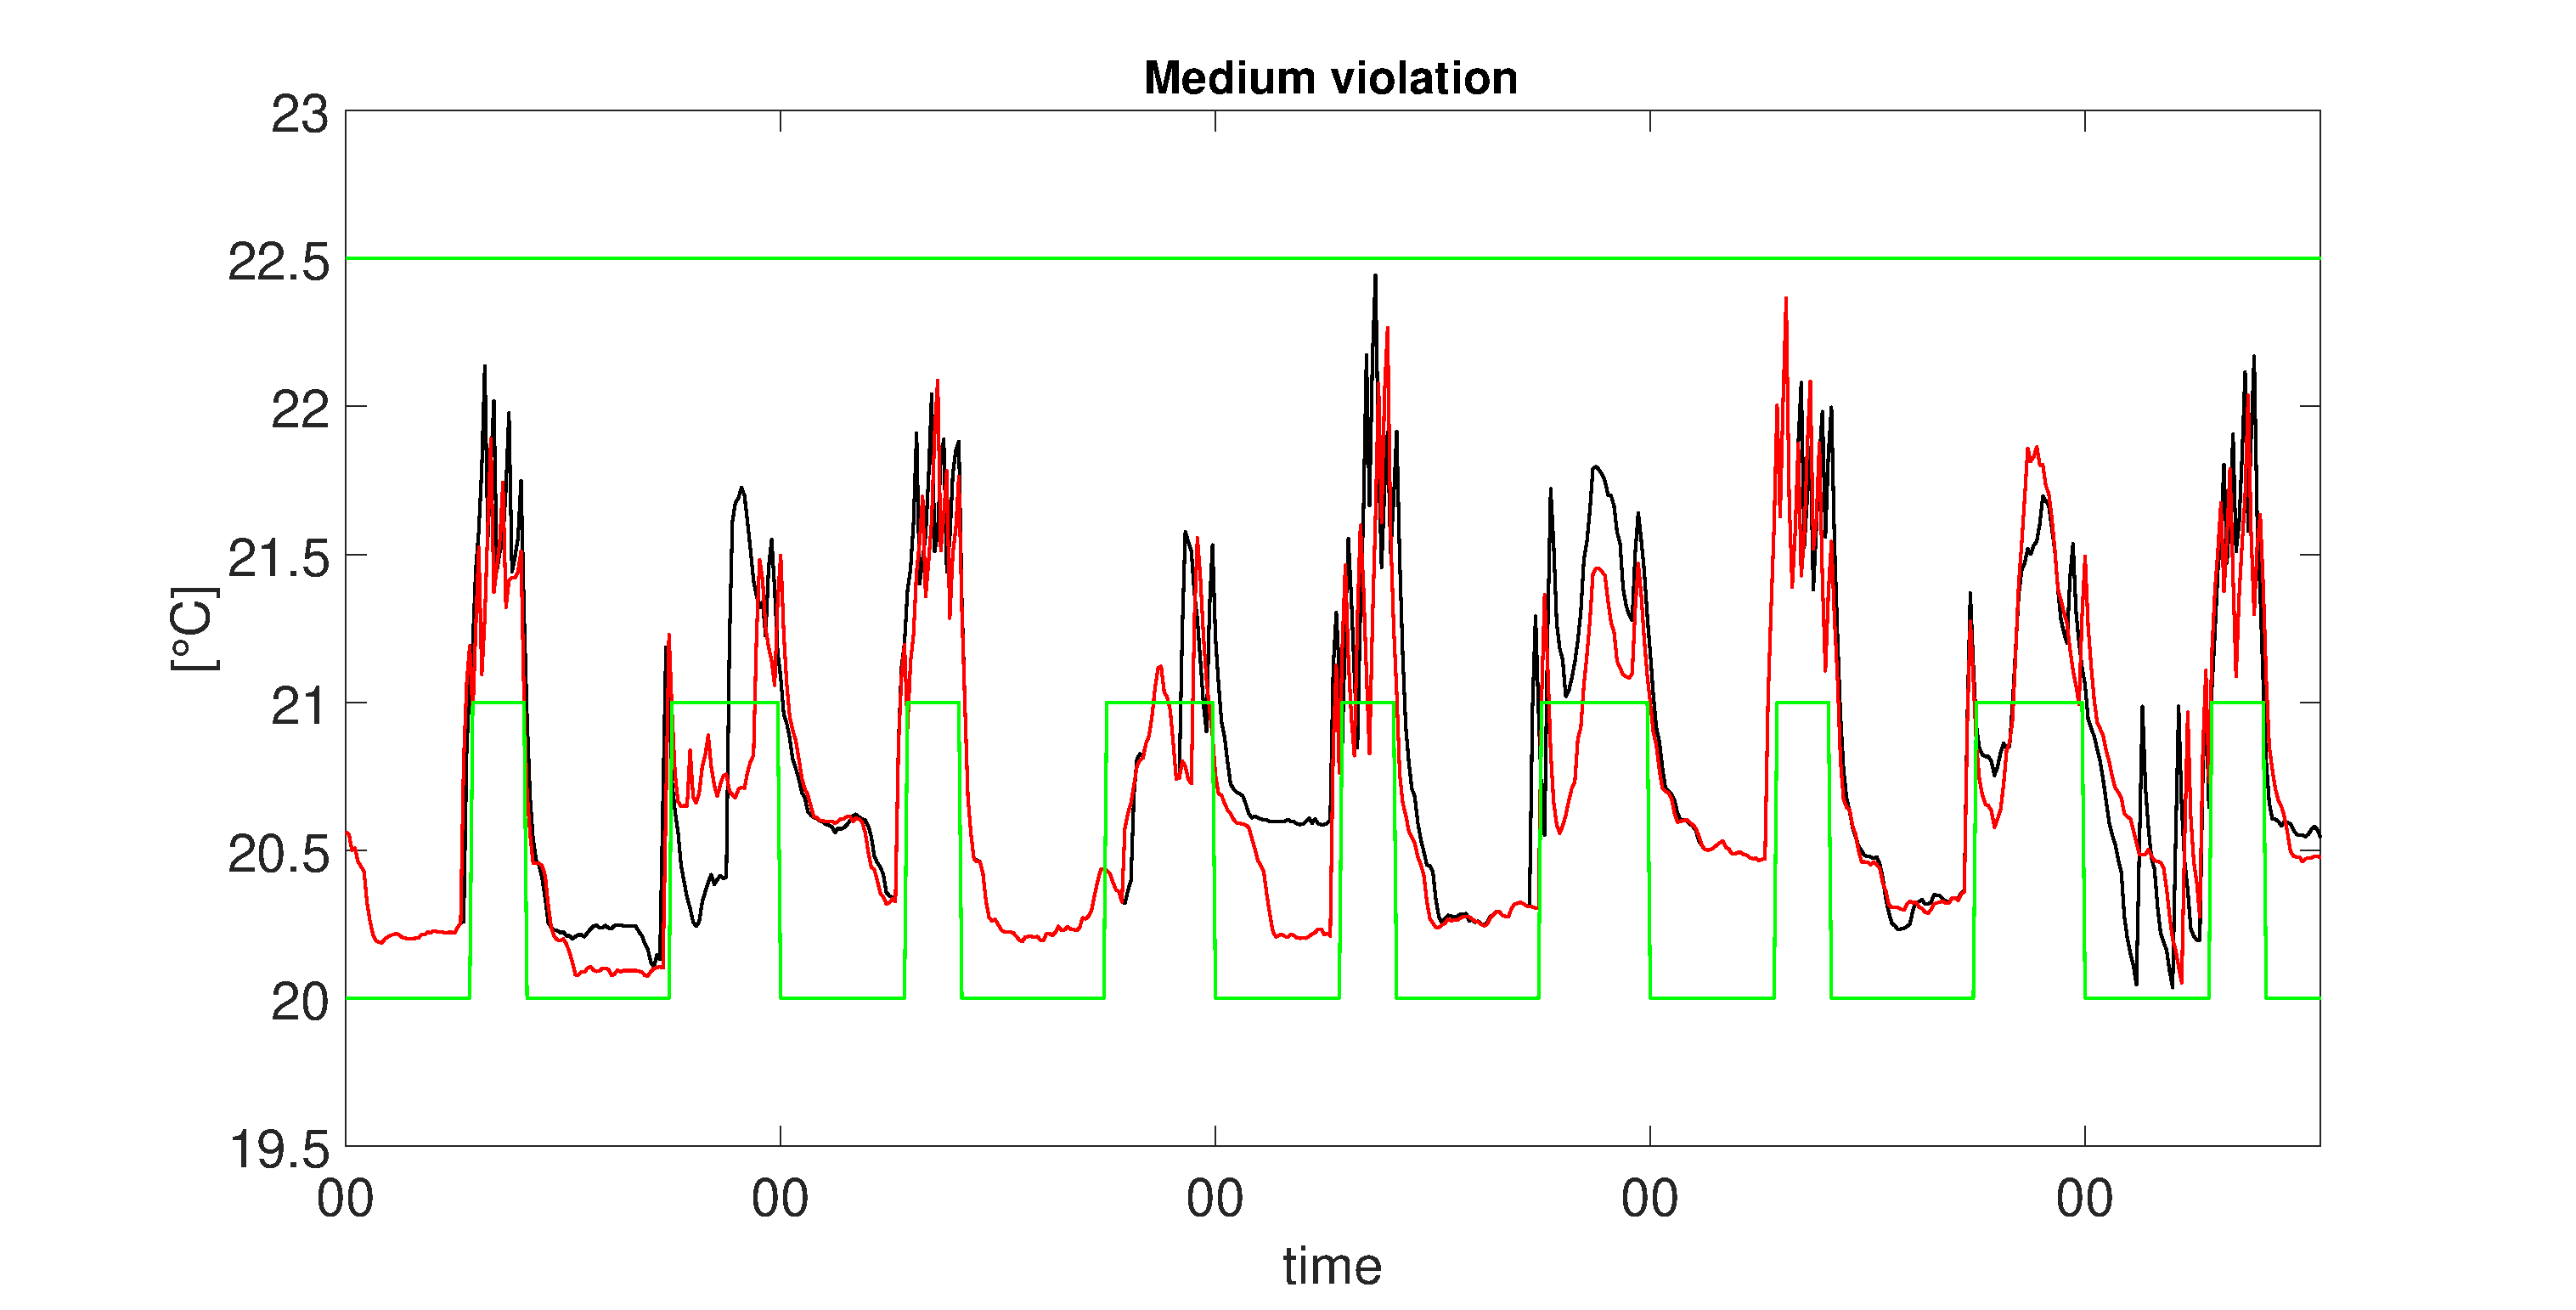
\includegraphics[width=23pc]{figures/Temperatures_medium_noisy.eps}
		}
		\subfigure{
			\label{F:LargeNoisy}
			\centering
			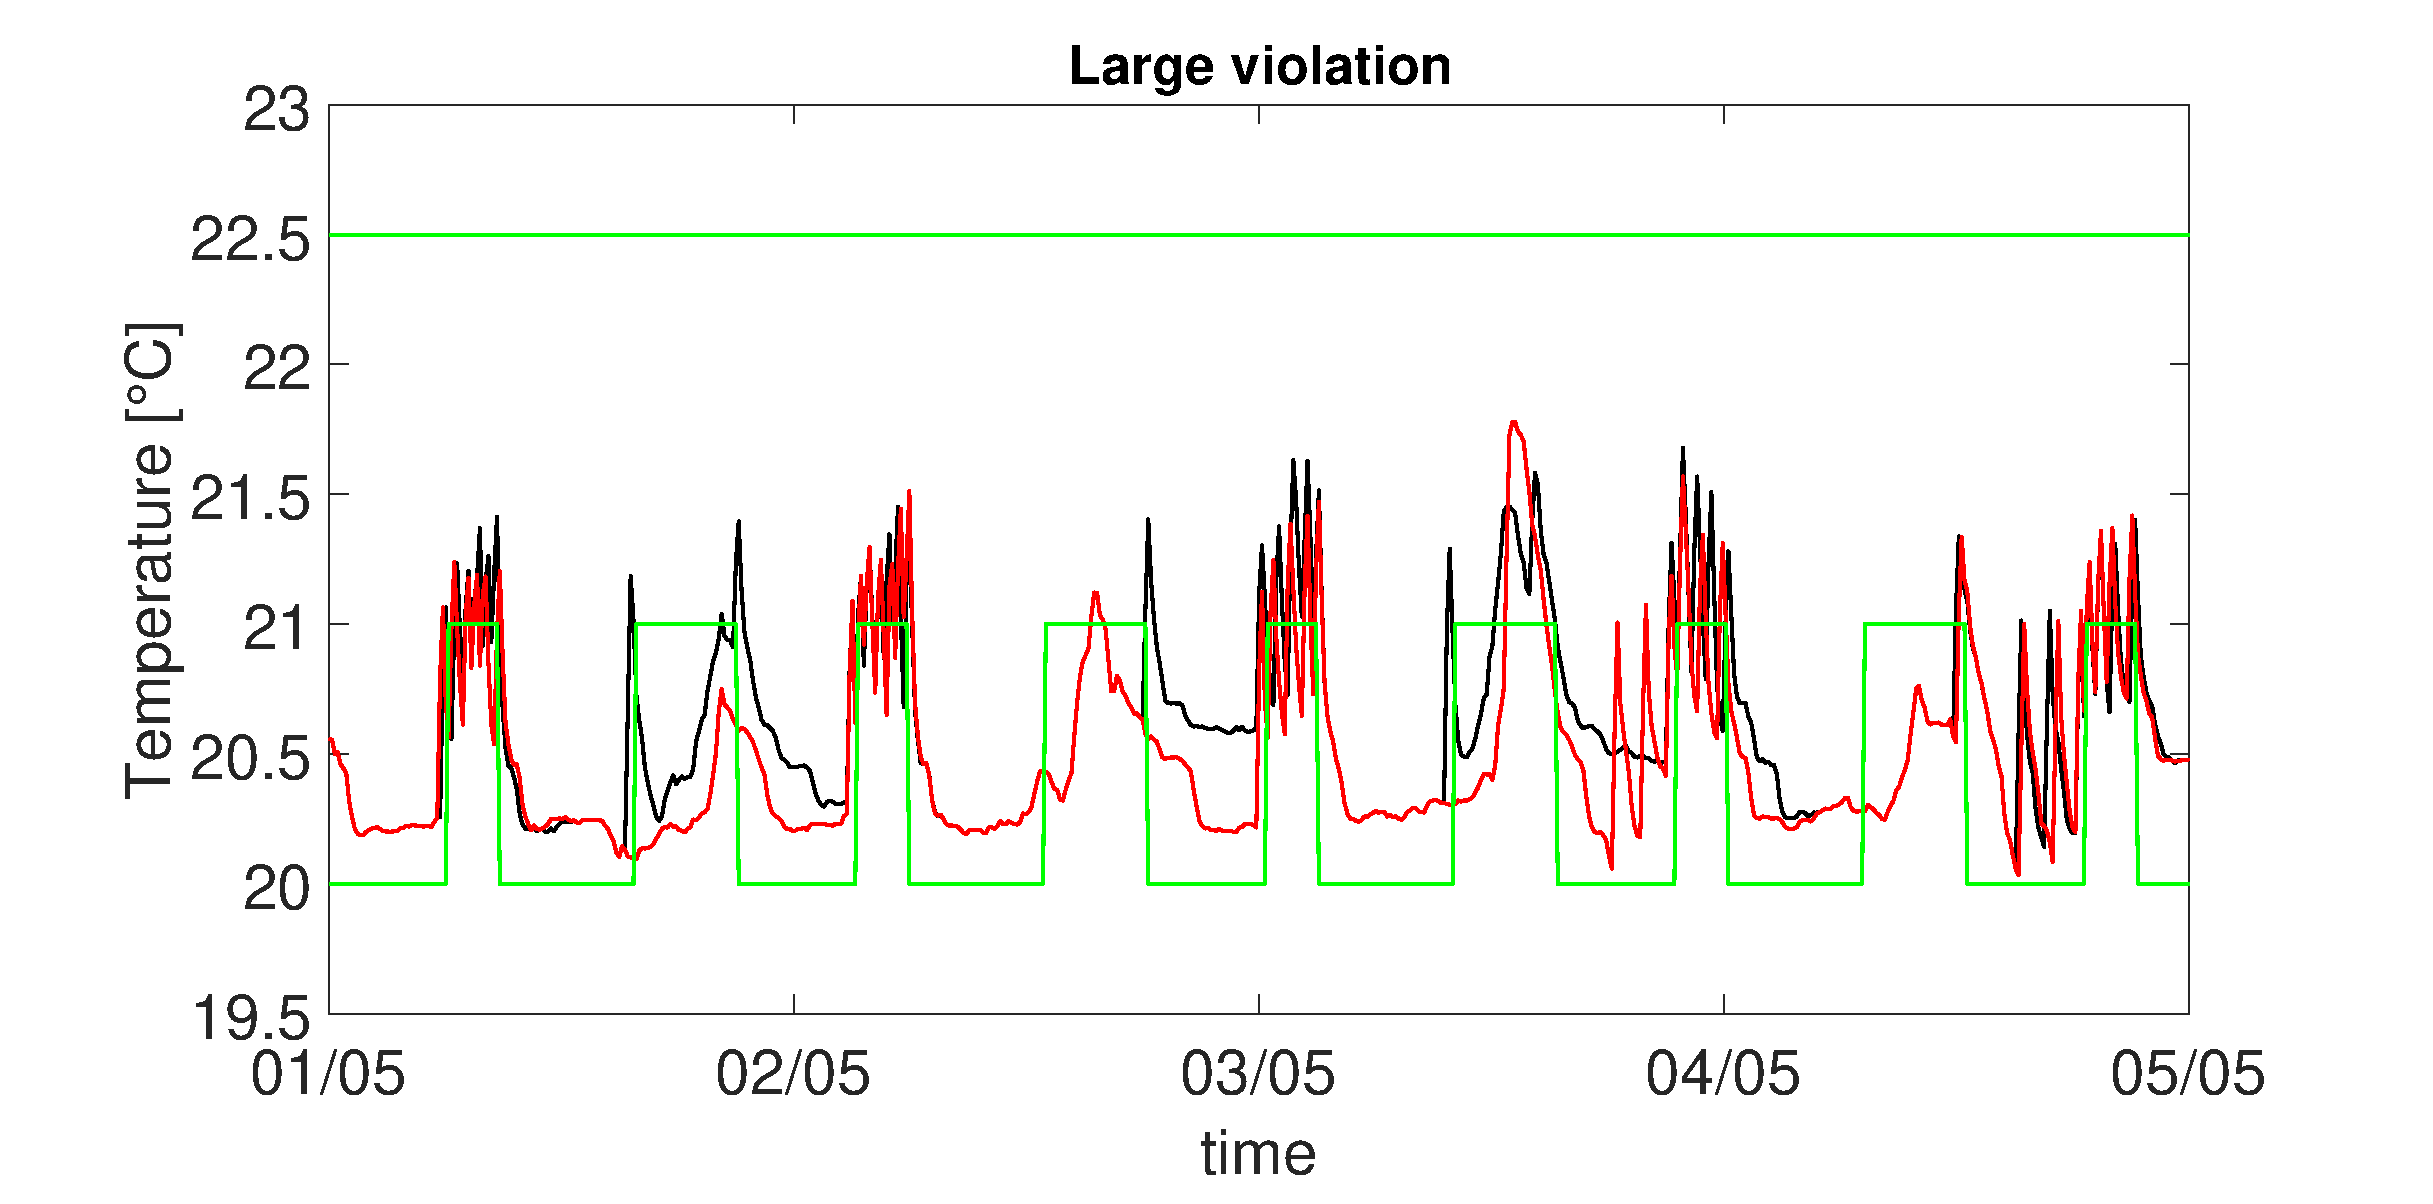
\includegraphics[width=23pc]{figures/Temperatures_large_noisy.eps}
		}	
	\end{center}
	\caption{\textcolor[rgb]{0,0,1}{Comparison of DPC considering perfect and noisy weather forecasts. Small, medium and large violation cases are compared.}}
	\captionsetup{justification=centering}
	\label{F:ComparisonTempNoisy}
\end{figure}

\begin{table}[t!]
	\centering
	%	\scalebox{0.9}{
	\textcolor[rgb]{0,0,1}{\begin{tabular}{lccccc}
		\toprule
		CONTROLLER  & LBV $\mathrm{MBE}$  & LBV $\mathrm{RMSE}$ & UBV $\mathrm{MBE}$ & UBV $\mathrm{RMSE}$ 	\\ 
		\midrule
		$DPC-SV$    & $0.034$             & $0.142$  			      & $0$    				 & $0$     	  	\\
		$DPC-MV$    & $0.178$ 			  & $0.453$       			  & $0$    				 & $0$		  	\\
		$DPC-LV$    & $0.478$  			  & $0.891$     			  & $0$    				 & $0$	      	\\
		\bottomrule
	\end{tabular}}
	%	}
	\caption{\textcolor[rgb]{0,0,1}{Lower Bound Violation (LBV) and Upper Bound Violation (UBV) errors expressed as $\mathrm{MBE}\%$ and $\mathrm{CV(RMSE)}\%$ for DPC Small Violation (DPC-SV), DPC Medium Violation (DPC-MV), DPC large Violation (DPC-LV) and bang-bang controller, considering noisy weather forecast.}}
	\captionsetup{justification=centering}
	\label{T:violationErrorsNoisy}
\end{table}


\textcolor[rgb]{0,0,1}{\paragraph{Result 2} 
In Figure \ref{F:comparison_all_energy_E+_noisy}, we show the difference in terms of energy consumption considering the perfect weather forecast (full line) and the noisy one (dashed line).
We can observe that the case with imperfect forecast is very close to the perfect forecast case.
We recall that we are optimizing a weighted sum of energy and thermal comfort, so depending on the conditions for which the disturbance is over or underestimated, the MPC can require to use more or less energy to supply the prediction errors.
In the small violation case, the energy consumption of the 2 conditions is closer than in the others.
This is because the DPC keeps the temperature within the bounds with an extremely small error in bounds violation.
In particular, the only exception can be seen before May $3^{rd}$ (03/05), where, due to the prediction error, the temperature violates the bounds, so the control uses more energy (than the perfect case) to bring it back above the threshold.
In the other 2 cases, when the temperature violates the bounds, due to the fact that violation constraints are more relaxed, the DPC does not require a too big control effort, hence using less energy.}

\textcolor[rgb]{0,0,1}{These results show the strong robustness of the DPC with respect to errors in the weather forecast.}
\begin{figure}[t!]
	\begin{center}
		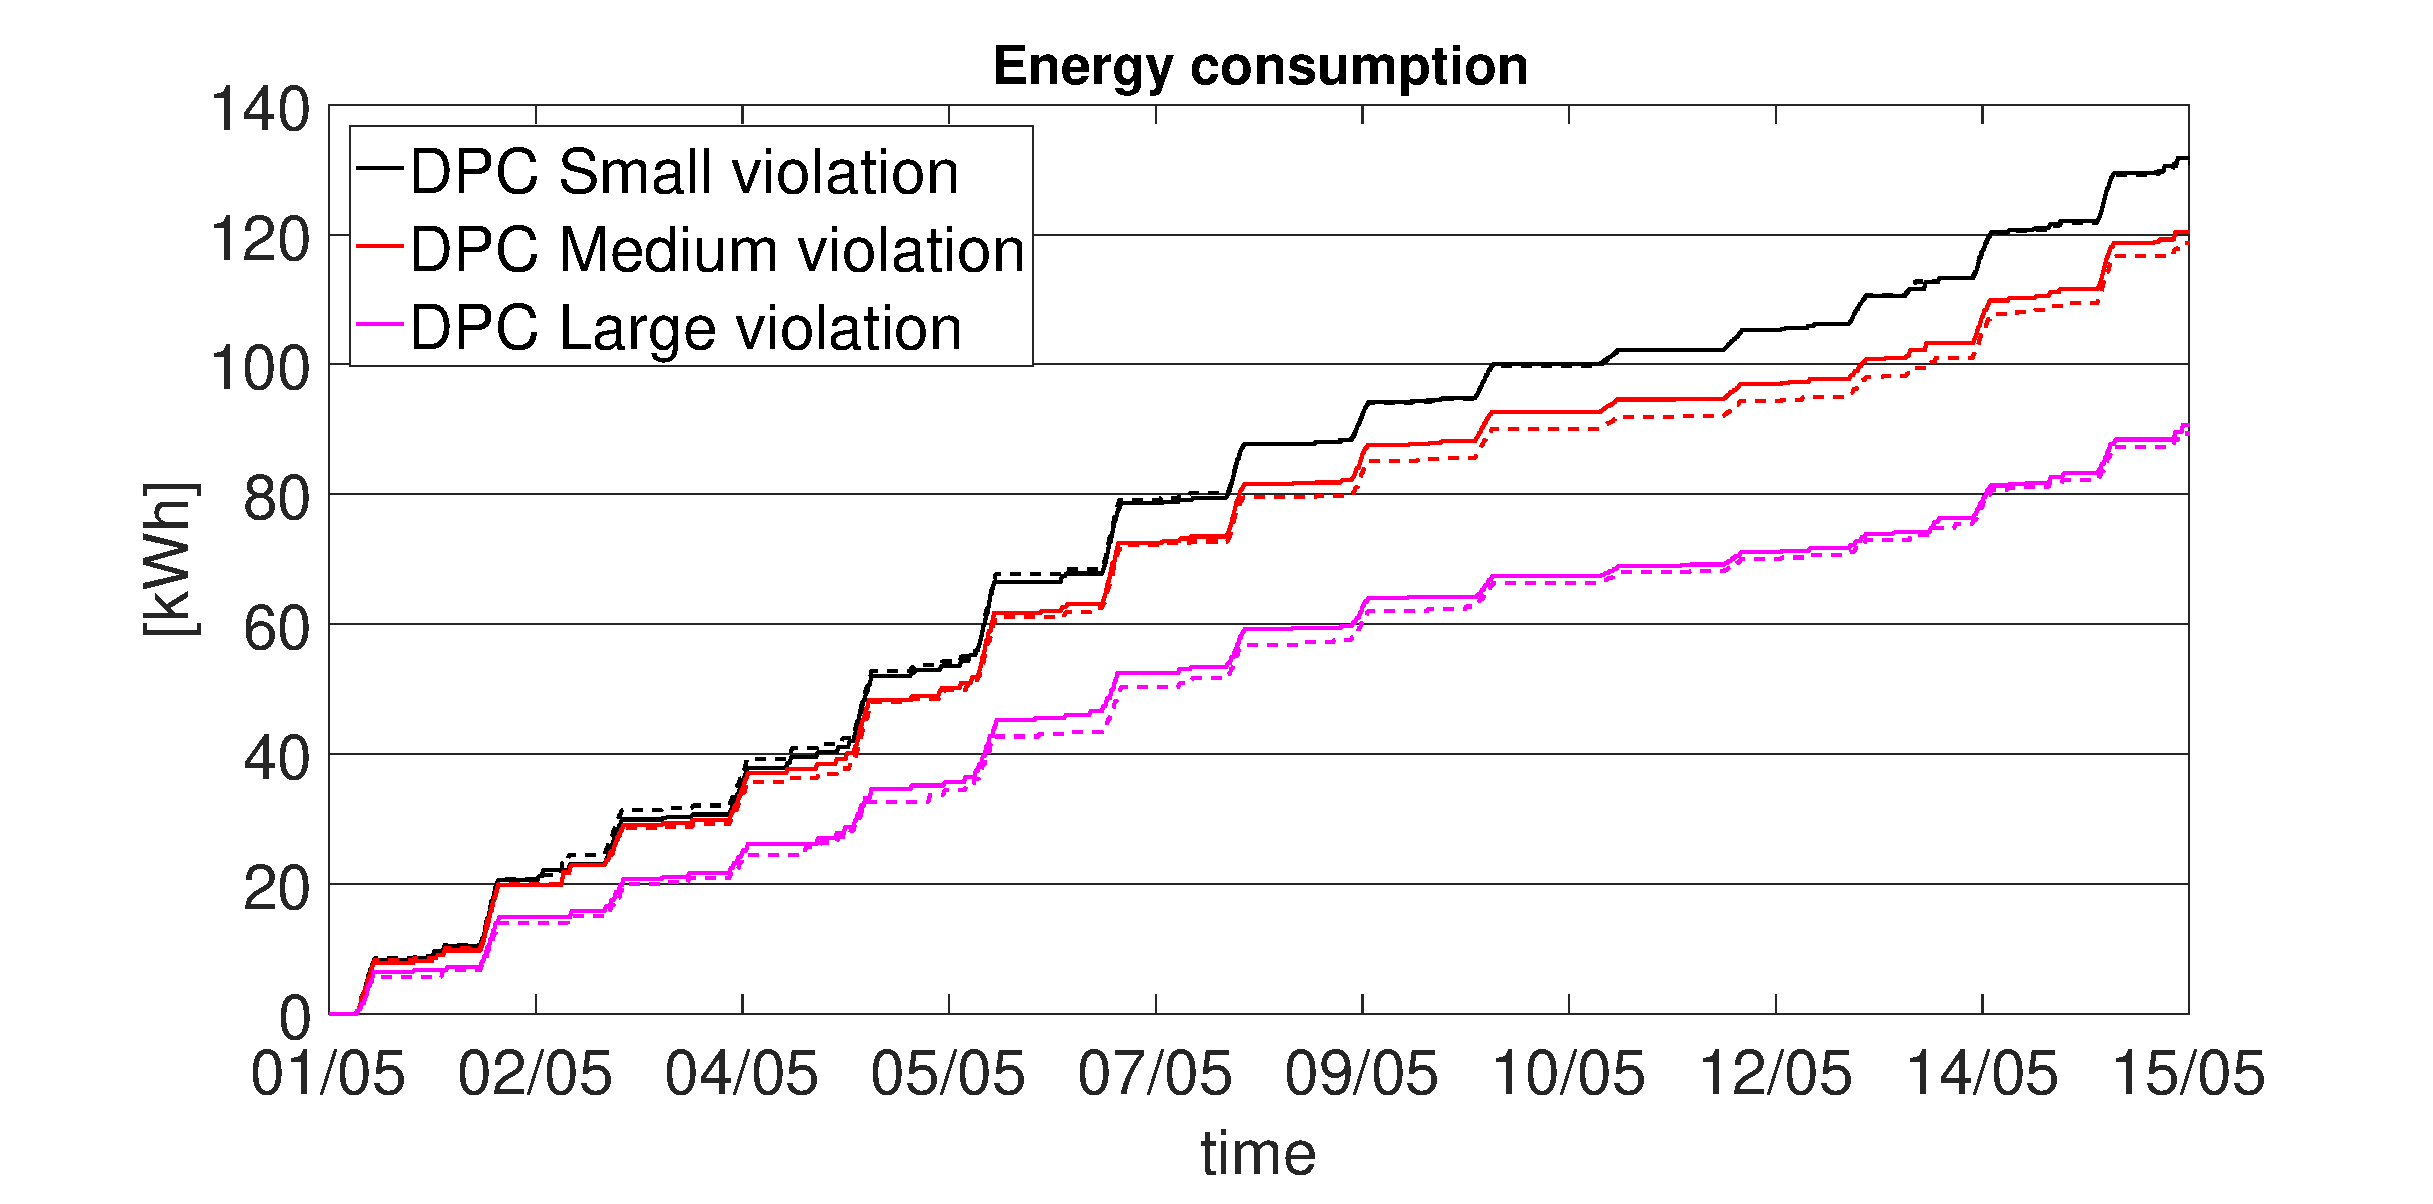
\includegraphics[width=28pc]{figures/Energy_all_EnergyPlus_noisy.eps}
	\end{center}
	\caption{\textcolor[rgb]{0,0,1}{Comparison of DPC in terms of thermal energy saving using EnergyPlus model, considering perfect (full) and imperfect (dashed) weather forecast, over $15$ days of the testing period with different violation configurations. The performance are pretty similar, showing the potential robustness of DPC.}}
	\label{F:comparison_all_energy_E+_noisy}
\end{figure}
